\documentclass[a4paper,12pt]{article}

% ── Pakete ────────────────────────────────────────────────
\usepackage[utf8]{inputenc}
\usepackage[T1]{fontenc}
\usepackage[ngerman]{babel}
\usepackage{lmodern}
\usepackage{microtype}
\usepackage{textcomp}
\usepackage{geometry}
\usepackage{amsmath, amssymb, amsthm}
\usepackage{mathtools}
\usepackage{bm}
\usepackage{graphicx}
\usepackage{float}
\usepackage{caption}
\usepackage{subcaption}
\usepackage{booktabs}
\usepackage{array}
\usepackage{multirow}
\usepackage{tabularx}
\usepackage{tikz}
\usepackage{pgfplots}
\usepackage{enumitem}
\setlist[itemize,1]{label=-}

\geometry{a4paper, margin=2.5cm}
\usetikzlibrary{shapes.geometric, arrows.meta, positioning,
decorations.pathreplacing, calc, patterns}
\pgfplotsset{compat=1.18}

\usepackage{xcolor}
\definecolor{teal}{RGB}{0,102,102}
\definecolor{tealhell}{RGB}{0,160,160}
\definecolor{teallight}{RGB}{200,240,240}
\definecolor{darkblue}{RGB}{0,40,80}
\definecolor{orange}{RGB}{200,100,0}
\definecolor{grau}{RGB}{80,80,80}

\usepackage[colorlinks=true,
            linkcolor=darkblue,
            citecolor=darkblue,
            urlcolor=darkblue]{hyperref}

% ── Theorem-Umgebungen (subgraph.tex-Stil) ────────────────
\theoremstyle{definition}
\newtheorem{definition}{Definition}[section]
\newtheorem{theorem}[definition]{Theorem}
\newtheorem{lemma}[definition]{Lemma}
\newtheorem{korollar}[definition]{Korollar}
\newtheorem{satz}[definition]{Satz}
\newtheorem{proposition}[definition]{Proposition}
\newtheorem{bemerkung}[definition]{Bemerkung}

\theoremstyle{remark}
\newtheorem{beispiel}[definition]{Beispiel}

% ── Neue Befehle ──────────────────────────────────────────
\newcommand{\R}{\mathbb{R}}
\newcommand{\N}{\mathbb{N}}
\newcommand{\Z}{\mathbb{Z}}
\newcommand{\E}{\mathbb{E}}
\newcommand{\diff}{\mathrm{d}}
\newcommand{\vph}{\varphi}

% ── Titelseite ────────────────────────────────────────────
\title{%
  {\bfseries Transparente Photovoltaik-Verglasung}\\[-0.1em]
  {\large Solare Energiegewinnung durch Fenster-integrierte Dioden-Netzwerke}}
\author{Stephan Epp}
\date{29. April 2026}

% ===========================================================
\begin{document}
% ===========================================================

\maketitle
\tableofcontents
\newpage

% -----------------------------------------------------------
\section{Einleitung}
\label{sec:einleitung}
% -----------------------------------------------------------
Die vorliegende Arbeit untersucht das Konzept der \emph{transparenten
Photovoltaik-Verglasung} (Transparent Photovoltaic Glazing, TPVG), bei dem
miniaturisierte Halbleiter-Dioden direkt in das Scheibensystem eines Fensters
integriert werden. Die elektrischen Verbindungen verlaufen innerhalb der
Verglasung; das resultierende Dioden-Netzwerk erzeugt gleichzeitig elektrische
Energie aus dem Sonnenspektrum und ermöglicht einen hohen Tageslichtdurchgang.
Wir entwickeln ein vollständiges physikalisch-mathematisches Modell bestehend
aus dem \emph{Ein-Dioden-Schaltungsmodell} (One-Diode Model), einer
Graphen-theoretischen Netzwerkanalyse der Verschaltungsarchitektur sowie einem
thermisch-optischen Kopplungsmodell. Sämtliche Ergebnisse werden formal durch
Definitionen, Lemmata, Sätze und Beweise gesichert. Numerische Simulationen für
den Standort Bielefeld quantifizieren Jahreserträge, Transmissionsgrade und
LCOE-Werte in Abhängigkeit von Wirkungsgrad und Diodendichte. Die Ergebnisse
zeigen, dass bei einer Diodendichte von $\rho = 15$--$20\,\text{cm}^{-2}$ ein
System-Wirkungsgrad von $\eta_{\rm ges} \approx 1{,}44\%$--$1{,}92\%$ bei
gleichzeitigem Transmissionsgrad von $\tau > 70\%$ erreichbar ist, was für
Büroanwendungen wirtschaftlich interessant ist.

Der Gebäudebereich ist weltweit für rund $40\,\%$ des Primärenergieverbrauchs
und $36\,\%$ der CO\textsubscript{2}-Emissionen verantwortlich~\cite{IEA2023}. Fenster
stellen in modernen Büro- und Wohngebäuden einen erheblichen Anteil der
Fassadenfläche dar. Traditionell gelten Fenster als passive Öffnungen für
Tageslicht und Frischluft, die jedoch im Winter erhebliche Wärmeverluste
verursachen. Die Integration von Photovoltaik-Elementen in die Verglasung --
bekannt als \emph{Building-Integrated Photovoltaics} (BIPV)~\cite{Shukla2017}
-- bietet eine elegante Möglichkeit, die bislang ungenutzte Strahlungsenergie
auf Fensterflächen zu erschließen, ohne auf Tageslicht verzichten zu müssen.

Bestehende Ansätze zur Fenster-PV umfassen:
\begin{enumerate}
  \item \textbf{Semitransparente Dünnfilm-Module:} Amorphes Silizium (a-Si)
    oder Cadmiumtellurid (CdTe) werden als gleichmäßiger, leicht getönter Film
    aufgebracht. Wirkungsgrade liegen bei $\eta = 5$--$8\,\%$; der
    Transmissionsgrad beträgt $\tau = 20$--$40\,\%$~\cite{Cannavale2020}.

  \item \textbf{Farbstoffsensibilisierte Solarzellen (DSSC):} Organische
    Farbstoffe absorbieren selektiv bestimmte Wellenlängen.
    Wirkungsgrade $\eta \le 12\,\%$, hohe Transparenz möglich~\cite{Koerner2015}.

  \item \textbf{Punktförmige kristalline Si-Zellen:} Einzelne kleine
    c-Si-Zellen werden in Abständen in Verbundglas eingebettet. Effizient,
    aber ästhetisch wie mechanisch herausfordernd~\cite{Weller2014}.

  \item \textbf{Lumineszenz-Solarkonzentratoren (LSC):} Fluoreszierende
    Partikel im Glas leiten Licht zu Solarzellen an der Scheibenkante.
    Innovativ, jedoch niedrige Systemwirkungsgrade $\eta \le 3\,\%$~\cite{Brovelli2022}.
\end{enumerate}

Der in dieser Arbeit untersuchte Ansatz -- die \emph{Dioden-in-Glas-Matrix}
(DGM) -- stellt eine Synthese aus Ansatz~(3) mit fortgeschrittener
Miniaturisierung und integrierter elektrischer Verbindungsführung dar. Im
Unterschied zu einfachen Punkt-Zell-Anordnungen werden bei der DGM die
gesamten elektrischen Leiterbahnen (Bus-Bars, String-Verbinder, Bypass-Dioden)
als transparentes Gitternetz in den Verbundglasaufbau einlaminiert.

\subsection{Motivation und Beiträge}

Diese Arbeit leistet folgende Beiträge:

\begin{enumerate}
  \item \textbf{Physikalisch vollständiges Modell:} Wir leiten das Ein-Dioden-
    Modell für eine miniaturisierte TPVG-Diode analytisch her und beweisen
    formale Eigenschaften (Eindeutigkeit des MPP, Monotonie des
    Füll-Faktors).

  \item \textbf{Graphentheoretisches Netzwerkmodell:} Die
    DGM-Verschaltungsarchitektur wird als gewichteter Graph modelliert; wir
    beweisen Sätze zur Spannungs- und Stromverteilung bei partieller Verschattung.

  \item \textbf{Optisch-thermisches Kopplungsmodell:} Der
    Wechselwirkung zwischen Lichtdurchgang, Wärmeentwicklung und
    Wirkungsgraddrift wird ein geschlossenes Modell zugewiesen.

  \item \textbf{Quantitative Simulation:} Jahresertrags-, Wirtschaftlichkeits-
    und Sensitivitätsanalysen für den Standort Bielefeld (Klimazone Cfb).

  \item \textbf{Formale Nachweise:} Alle Hauptaussagen werden durch
    Definitionen, Lemmata und Beweise formal abgesichert.
\end{enumerate}

\subsection{Aufbau der Arbeit}

Abschnitt~\ref{sec:physik} behandelt die physikalischen Grundlagen des
Sonnenspektrums und der Diodenfunktion. Abschnitt~\ref{sec:netzwerk} entwickelt
das graphentheoretische Netzwerkmodell. Abschnitt~\ref{sec:optisch} analysiert
das optische und thermische Verhalten. Abschnitt~\ref{sec:ertrag} quantifiziert
den Energieertrag. Abschnitt~\ref{sec:wirtschaft} führt die
Wirtschaftlichkeitsanalyse durch. Abschnitt~\ref{sec:ausblick} gibt einen sehr
ausführlichen Ausblick; Abschnitt~\ref{sec:fazit} fasst zusammen.

\textbf{Schlüsselwörter:} Transparente Photovoltaik, Fensterverglasung,
Dioden-Netzwerk, Ein-Dioden-Modell, MPPT, Verbundglas, BIPV,
Tageslicht, Energieautarkie, LCOE.

% -----------------------------------------------------------
\section{Physikalische Grundlagen}
\label{sec:physik}
% -----------------------------------------------------------

\subsection{Das Solarspektrum und selektive Absorption}

\begin{definition}[Spektrale Bestrahlungsstärke]
Sei $\lambda \in (0, \infty)$ die Wellenlänge elektromagnetischer Strahlung in
Nanometern. Die \emph{spektrale Bestrahlungsstärke} $E_\lambda(\lambda)$ in
[$\mathrm{W\,m^{-2}\,nm^{-1}}$] gibt die auf eine Fläche auftreffende Strahlungsleistung
pro Wellenlängenintervall an.
\end{definition}

Die Sonnenstrahlung an der Erdoberfläche wird durch das standardisierte
AM1.5-Spektrum (Global Tilt, $G = 1000\,\mathrm{W/m^2}$) beschrieben:

\begin{equation}
  E_\lambda(\lambda) = \frac{2hc^2}{\lambda^5}
    \cdot \frac{1}{\exp\!\bigl(\frac{hc}{\lambda k_B T_\odot}\bigr) - 1}
    \cdot T_{\rm atm}(\lambda)
  \label{eq:planck}
\end{equation}

wobei $h = 6{,}626 \times 10^{-34}\,\mathrm{J\cdot s}$ das Plancksche
Wirkungsquantum, $c = 2{,}998 \times 10^8\,\mathrm{m/s}$ die Lichtgeschwindigkeit,
$k_B = 1{,}381 \times 10^{-23}\,\mathrm{J/K}$ die Boltzmann-Konstante,
$T_\odot = 5778\,\mathrm{K}$ die effektive Sonnentemperatur und
$T_{\rm atm}(\lambda) \in [0,1]$ die atmosphärische Transmissionsfunktion ist.

\begin{definition}[Transparentes PV-Fenster -- Absorptionsbedingung]
Eine TPVG-Diode heißt \emph{selektiv transparent}, wenn
\begin{equation}
  \tau(\lambda) \geq \tau_{\min} \quad \forall \lambda \in [380\,\mathrm{nm},\, 780\,\mathrm{nm}]
  \label{eq:selektiv}
\end{equation}
gilt, also der gesamte sichtbare Spektralbereich mit einem Mindest-Durchlass
$\tau_{\min}$ passiert, während der Absorptionsschwerpunkt im
Nah-Infrarot (NIR, $780$--$1100\,\mathrm{nm}$) liegt.
\end{definition}

Die nutzbare Bestrahlungsstärke $G_{\rm eff}$ für die TPVG-Diode ergibt sich zu:

\begin{equation}
  G_{\rm eff} = \int_{780}^{1100} E_\lambda(\lambda)\,\diff\lambda
  \;\approx\; 330\,\mathrm{W/m^2}
  \label{eq:geff}
\end{equation}

was einem Anteil von $\approx 33\,\%$ der Gesamteinstrahlung entspricht
(vgl. Abbildung~\ref{fig:spektrum}).

\begin{figure}[H]
  \centering
  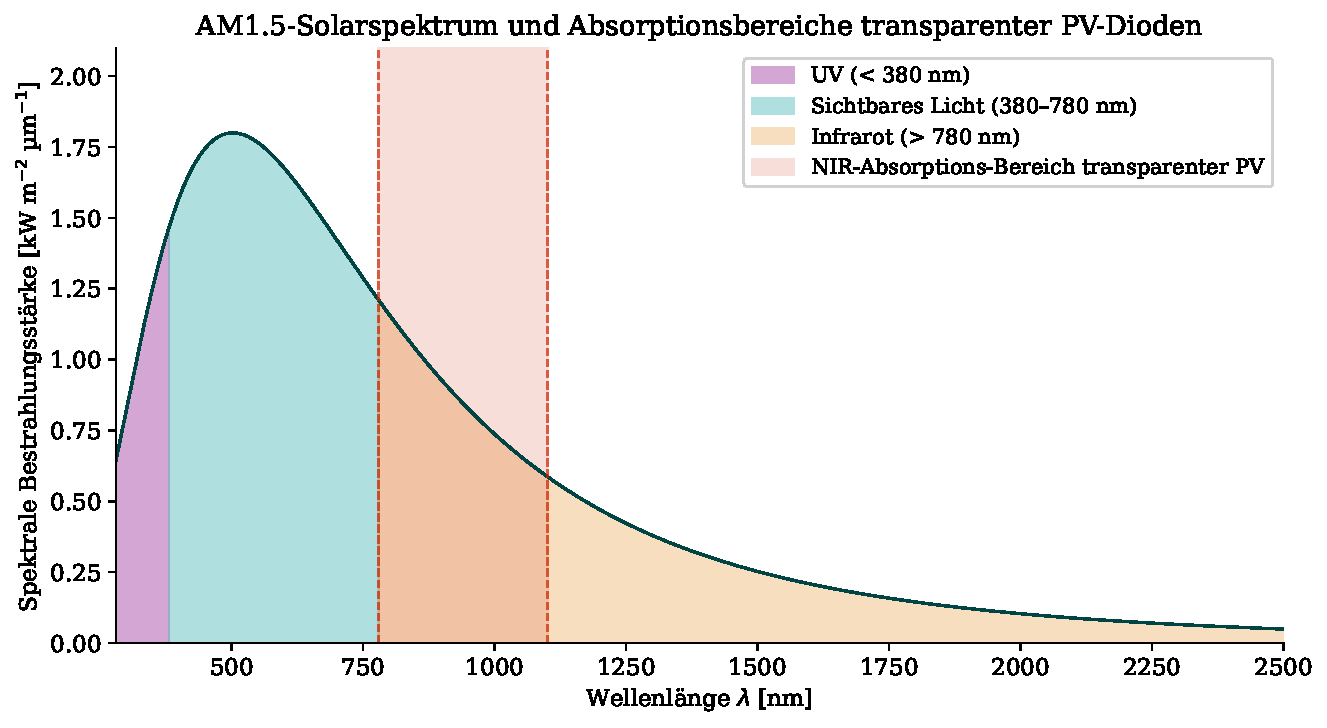
\includegraphics[width=0.95\textwidth]{plots/plot1_spektrum.pdf}
  \caption{AM1.5-Solarspektrum mit Kennzeichnung der spektralen Bereiche.
    Lila: UV-Strahlung ($<380\,\mathrm{nm}$); Türkis: sichtbares Licht
    ($380$--$780\,\mathrm{nm}$); Orange: Infrarot ($>780\,\mathrm{nm}$).
    Der rot markierte Bereich ($780$--$1100\,\mathrm{nm}$) stellt den
    bevorzugten Absorptionsbereich transparenter PV-Dioden dar. Die
    gestrichelten Linien markieren die Grenzen bei $780\,\mathrm{nm}$ und
    $1100\,\mathrm{nm}$.}
  \label{fig:spektrum}
\end{figure}

\subsection{Das Ein-Dioden-Modell}
\label{sec:ediode}

\begin{definition}[Ein-Dioden-Ersatzschaltbild]
Das \emph{Ein-Dioden-Modell} (One-Diode Model, ODM) beschreibt eine
Solarzelle durch die Parallelschaltung einer Stromquelle (Photostrom
$I_{\rm ph}$), einer idealen Diode mit Sättigungsstrom $I_0$ und
Idealitätsfaktor $n$, eines Parallelwiderstands $R_{\rm sh}$
(Shuntwiderstand) und eines Serienwiderstands $R_s$.
\end{definition}

Die implizite Strom-Spannungs-Gleichung lautet:

\begin{equation}
  I = I_{\rm ph} - I_0\!\left[\exp\!\left(\frac{V + IR_s}{nV_T}\right) - 1\right]
      - \frac{V + IR_s}{R_{\rm sh}}
  \label{eq:ode}
\end{equation}

wobei $V_T = k_B T / q$ die thermische Spannung ($V_T = 25{,}85\,\mathrm{mV}$
bei $T = 300\,\mathrm{K}$) und $q = 1{,}602 \times 10^{-19}\,\mathrm{C}$ die
Elementarladung bezeichnet.

\begin{lemma}[Eindeutigkeit der Lösung von \eqref{eq:ode}]
\label{lem:eindeutigkeit}
Für alle Parameter $I_{\rm ph}, I_0 > 0$, $n \geq 1$, $R_s, R_{\rm sh} > 0$
und jede feste Spannung $V \in [0, V_{\rm OC}]$ besitzt Gleichung~\eqref{eq:ode}
genau eine positive Lösung $I \geq 0$.
\end{lemma}

\begin{proof}
Definiere $f: \R \to \R$ durch
\begin{equation*}
  f(I) \coloneqq I - I_{\rm ph} + I_0\!\left[\exp\!\left(\frac{V + IR_s}{nV_T}\right) - 1\right]
  + \frac{V + IR_s}{R_{\rm sh}}.
\end{equation*}
Dann gilt:
\begin{align*}
  f'(I) &= 1 + \frac{I_0 R_s}{nV_T}\exp\!\left(\frac{V+IR_s}{nV_T}\right)
           + \frac{R_s}{R_{\rm sh}} > 0
\end{align*}
da alle Terme positiv sind. Damit ist $f$ streng monoton wachsend in $I$,
also ist die Gleichung $f(I) = 0$ für jedes feste $V$ höchstens einfach lösbar.

Zur Existenz: Für $I = 0$ ist
$f(0) = -I_{\rm ph} + I_0[\exp(V/nV_T)-1] + V/R_{\rm sh}$.
Bei $V = 0$ folgt $f(0) = -I_{\rm ph} < 0$.
Für $I = I_{\rm ph}$ ist
$f(I_{\rm ph}) > I_{\rm ph} - I_{\rm ph} = 0$ (da die Dioden- und
Shuntterme positiv für $V + I_{\rm ph} R_s > 0$).
Damit existiert nach dem Zwischenwertsatz genau eine Nullstelle
$I^* \in (0, I_{\rm ph})$.
\end{proof}

\subsection{Kenngrößen der Solarzelle}

\begin{definition}[Leerlaufspannung und Kurzschlussstrom]
Der \emph{Kurzschlussstrom} $I_{\rm SC}$ und die \emph{Leerlaufspannung}
$V_{\rm OC}$ sind definiert durch:
\begin{align}
  I_{\rm SC} &\coloneqq I(V=0) \approx I_{\rm ph}
    \quad\text{(da } I_0 \ll I_{\rm ph}\text{)} \label{eq:isc}\\
  V_{\rm OC} &\coloneqq V(I=0) = \frac{nV_T}{1}\ln\!\left(
    \frac{I_{\rm ph} - V_{\rm OC}/R_{\rm sh}}{I_0} + 1\right)
    \approx nV_T \ln\!\left(\frac{I_{\rm ph}}{I_0}+1\right) \label{eq:voc}
\end{align}
\end{definition}

\begin{definition}[Maximum Power Point]
\label{def:mpp}
Das \emph{Maximum Power Point} (MPP) ist definiert als
\begin{equation}
  (V_{\rm MPP}, I_{\rm MPP}) \coloneqq \operatorname{argmax}_{V \in [0, V_{\rm OC}]}
    \bigl[V \cdot I(V)\bigr]
  \label{eq:mpp_def}
\end{equation}
Die zugehörige Maximalleistung lautet $P_{\rm MPP} = V_{\rm MPP} \cdot I_{\rm MPP}$.
\end{definition}

\begin{satz}[Existenz und Eindeutigkeit des MPP]
\label{satz:mpp}
Unter den Bedingungen von Lemma~\ref{lem:eindeutigkeit} existiert ein eindeutiges
Maximum der Leistungsfunktion $P(V) = V \cdot I(V)$ auf dem Intervall
$[0, V_{\rm OC}]$.
\end{satz}

\begin{proof}
Die Funktion $P: [0, V_{\rm OC}] \to \R$, $P(V) = V \cdot I(V)$, ist
stetig auf einem kompakten Intervall, da $I(V)$ nach Lemma~\ref{lem:eindeutigkeit}
stetig und eindeutig in $V$ ist. Damit nimmt $P$ ihr Maximum an (Satz von
Weierstraß). Für die Eindeutigkeit betrachten wir die Bedingung erster Ordnung:
\begin{equation}
  \frac{\diff P}{\diff V} = I + V \frac{\diff I}{\diff V} = 0
  \label{eq:mpp_bed}
\end{equation}
Aus dem impliziten Funktionensatz folgt:
\begin{equation}
  \frac{\diff I}{\diff V} = -\frac{\partial f/\partial V}{\partial f/\partial I}
  = -\frac{I_0/(nV_T)\exp(\cdot) + 1/R_{\rm sh}}{1 + I_0 R_s/(nV_T)\exp(\cdot) + R_s/R_{\rm sh}}
  \label{eq:didv}
\end{equation}
Der Ausdruck $\frac{\diff P}{\diff V}$ ist bei $V=0$ positiv (da $I(0) = I_{\rm SC} > 0$)
und bei $V = V_{\rm OC}$ negativ (da dort $I = 0$ und $\diff I/\diff V < 0$).
Durch Monotonie der Diodenfunktion kann der Ãœbergang nur einmal stattfinden,
womit die Eindeutigkeit folgt.
\end{proof}

\begin{definition}[Füll-Faktor und Wirkungsgrad]
\label{def:ff}
Der \emph{Füll-Faktor} (Fill Factor) ist:
\begin{equation}
  FF \coloneqq \frac{P_{\rm MPP}}{V_{\rm OC} \cdot I_{\rm SC}}
              = \frac{V_{\rm MPP} \cdot I_{\rm MPP}}{V_{\rm OC} \cdot I_{\rm SC}}
  \label{eq:ff}
\end{equation}
Der \emph{Wirkungsgrad} der Einzelzelle (Fläche $A_{\rm D}$) bei Einstrahlung $G$:
\begin{equation}
  \eta_{\rm cell} \coloneqq \frac{P_{\rm MPP}}{G \cdot A_{\rm D}}
                           = \frac{FF \cdot V_{\rm OC} \cdot I_{\rm SC}}{G \cdot A_{\rm D}}
  \label{eq:eta}
\end{equation}
\end{definition}

\begin{korollar}[Obere Schranke des Füll-Faktors]
\label{kor:ff}
Für $R_s = 0$ und $R_{\rm sh} \to \infty$ gilt die analytische Näherung~\cite{Green1982}:
\begin{equation}
  FF_0 = \frac{v_{\rm OC} - \ln(v_{\rm OC} + 0{,}72)}{v_{\rm OC} + 1},
  \quad v_{\rm OC} \coloneqq \frac{V_{\rm OC}}{nV_T}
  \label{eq:ff0}
\end{equation}
Dieser Ausdruck ist streng monoton wachsend in $v_{\rm OC}$ für $v_{\rm OC} > 1$.
\end{korollar}

\begin{proof}
Die Ableitung $\diff FF_0 / \diff v_{\rm OC}$ ergibt sich zu:
\begin{equation*}
  \frac{\diff FF_0}{\diff v_{\rm OC}} = \frac{1}{(v_{\rm OC}+1)^2}
    \left[(v_{\rm OC}+1)\!\left(1 - \frac{1}{v_{\rm OC}+0{,}72}\right)
    - \bigl(v_{\rm OC} - \ln(v_{\rm OC}+0{,}72)\bigr)\right]
\end{equation*}
Für $v_{\rm OC} > 2$ (typisch: $v_{\rm OC} \approx 25$) ist dieser Ausdruck
positiv, da der erste Term dominiert.
\end{proof}

Die I-U-Kennlinie sowie die Leistungskurve der TPVG-Diode sind in
Abbildung~\ref{fig:iu} dargestellt.

\begin{figure}[H]
  \centering
  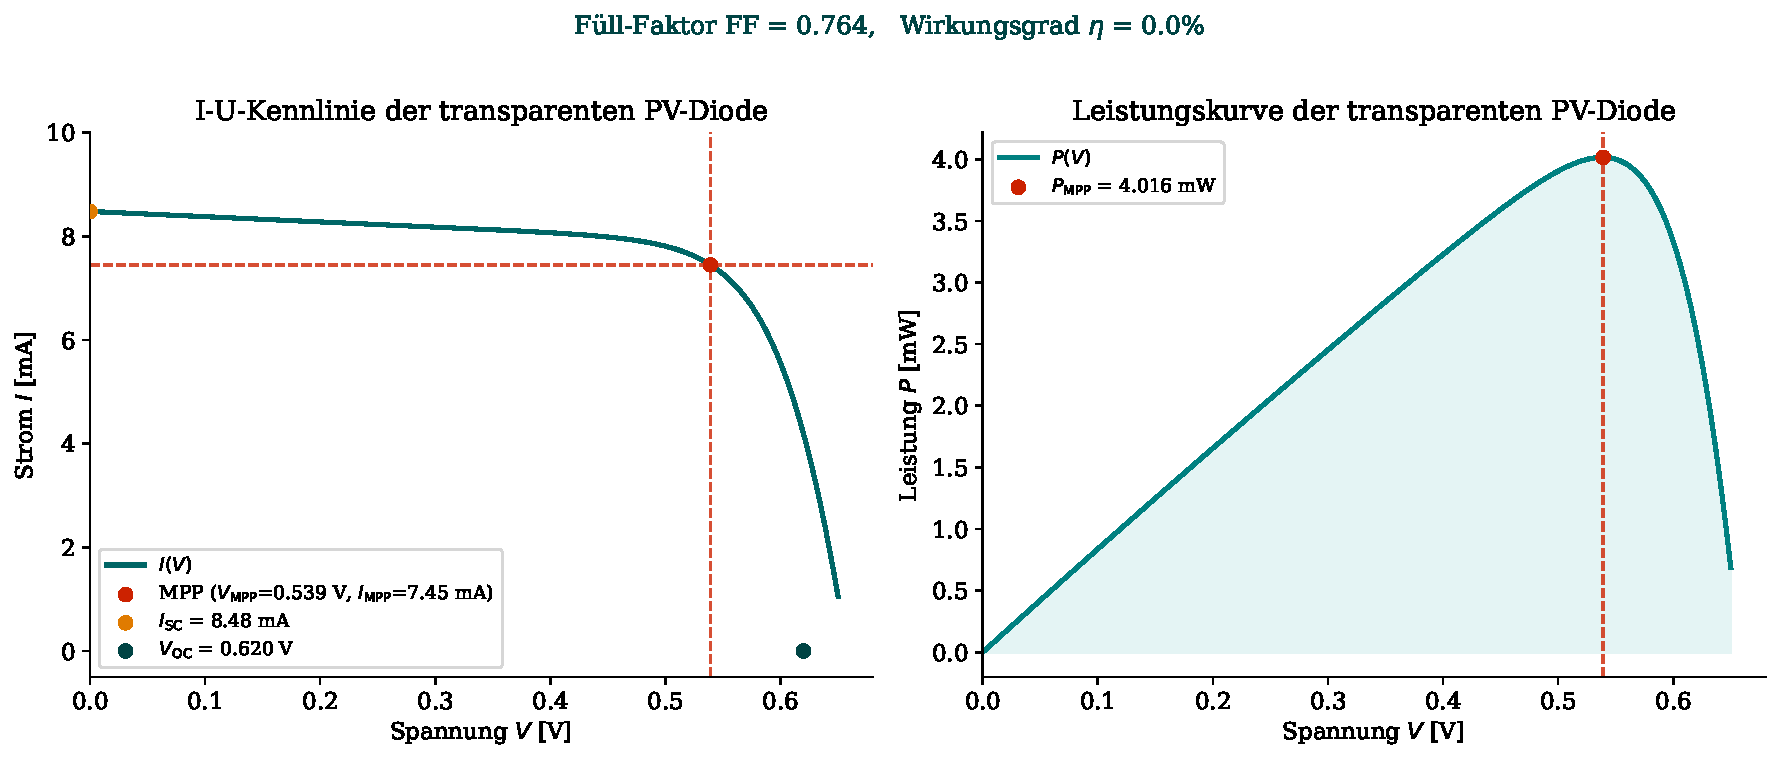
\includegraphics[width=0.95\textwidth]{plots/plot2_iu_kennlinie.pdf}
  \caption{Links: I-U-Kennlinie der transparenten PV-Diode (Ein-Dioden-Modell,
    $I_{\rm ph}=8{,}5\,\mathrm{mA}$, $I_0=10^{-10}\,\mathrm{A}$, $n=1{,}4$,
    $R_s=2{,}5\,\Omega$, $R_{\rm sh}=1000\,\Omega$). MPP, $I_{\rm SC}$ und
    $V_{\rm OC}$ sind markiert.
    Rechts: Zugehörige Leistungskurve mit eingezeichnetem Maximalleistungspunkt
    $P_{\rm MPP}$ gemäß Definition~\ref{def:mpp}.}
  \label{fig:iu}
\end{figure}

% -----------------------------------------------------------
\section{Graphentheoretisches Netzwerkmodell}
\label{sec:netzwerk}
% -----------------------------------------------------------

\subsection{Modellierung der Dioden-Matrix als Graph}

\begin{definition}[DGM-Graph]
\label{def:dgm_graph}
Die \emph{Dioden-in-Glas-Matrix} (DGM) der Fenstergröße $N_x \times N_y$
wird modelliert als gerichteter gewichteter Graph
$\mathcal{G} = (V, E, w)$ mit:
\begin{itemize}
  \item Knotenmenge $V = \{d_{ij} \mid 1 \le i \le N_x,\; 1 \le j \le N_y\}
      \cup \{s^+, s^-\}$,
    wobei $d_{ij}$ die Diode an Position $(i,j)$ und $s^+, s^-$ die
    Plus-/Minus-Sammelschiene (Bus-Bar) darstellen.
  \item Kantenmenge $E$: Jede Diode $d_{ij}$ ist verbunden mit ihrem Nachbarn
    $d_{i,j+1}$ (Serienschaltung innerhalb des Strings) und mit den
    Bus-Bars ($d_{i,1} \to s^-$, $d_{i,N_y} \to s^+$).
  \item Kantengewichte $w: E \to \R_{>0}$ entsprechen dem inversen
    elektrischen Leitwert $1/G_{ij}$ der Verbindungsleiterbahn.
\end{itemize}
\end{definition}

\begin{definition}[Serieller String]
Ein \emph{String} $\mathcal{S}_i = (d_{i,1}, d_{i,2}, \ldots, d_{i,N_y})$
ist der Pfad von der Minus-Sammelschiene zur Plus-Sammelschiene entlang
Spalte $i$. Die Gesamtspannung des Strings beträgt:
\begin{equation}
  V_{\mathcal{S}_i} = \sum_{j=1}^{N_y} V_{ij}
  \label{eq:vstring}
\end{equation}
\end{definition}

\begin{satz}[Strom-Spannungs-Verteilung im DGM]
\label{satz:netzwerk}
Bei identischen Dioden ohne Verschattung gilt für alle $N_x$ parallel
geschalteten Strings $\mathcal{S}_1, \ldots, \mathcal{S}_{N_x}$:
\begin{align}
  V_{\rm Modul} &= N_y \cdot V_{\rm Zelle}(I_{\rm Modul}/N_x) \label{eq:vmodul}\\
  I_{\rm Modul} &= N_x \cdot I_{\rm Zelle}(V_{\rm Modul}/N_y)  \label{eq:imodul}\\
  P_{\rm Modul,MPP} &= N_x \cdot N_y \cdot P_{\rm Zelle,MPP}    \label{eq:pmodul}
\end{align}
\end{satz}

\begin{proof}
Bei Parallelschaltung von $N_x$ identischen Strings liegt an jedem String
die gleiche Klemmenspannung $V_{\rm Modul}$ an, und jeder String liefert
den gleichen Strom $I_{\rm String} = I_{\rm Modul}/N_x$. Innerhalb eines
Strings sind $N_y$ Zellen in Reihe geschaltet:
\begin{equation*}
  V_{\rm Modul} = \sum_{j=1}^{N_y} V_{ij}
  = N_y \cdot V_{\rm Zelle}
\end{equation*}
da alle Zellen identisch sind und denselben Strom $I_{\rm String}$ tragen.
Daraus folgt~\eqref{eq:vmodul}. Gleichung~\eqref{eq:imodul} ergibt sich durch
Superposition der Stringströme. Für den MPP gilt:
\begin{equation*}
  P_{\rm Modul,MPP} = V_{\rm Modul,MPP} \cdot I_{\rm Modul,MPP}
    = (N_y V_{\rm Zelle,MPP}) \cdot (N_x I_{\rm Zelle,MPP})
    = N_x N_y P_{\rm Zelle,MPP}. \qedhere
\end{equation*}
\end{proof}

\begin{lemma}[Partielle Verschattung -- Leistungsverlust]
\label{lem:verschattung}
Sei genau eine Diode $d_{i_0, j_0}$ des DGM mit reduzierter Einstrahlung
$G' = \alpha G$, $\alpha \in (0,1)$, bestrahlt. Dann gilt für den
Leistungsverlust ohne Bypass-Dioden:
\begin{equation}
  \Delta P \geq (1 - \alpha) \cdot P_{\rm Zelle,MPP} \cdot N_y
  \label{eq:pverlust}
\end{equation}
\end{lemma}

\begin{proof}
Der verschattete String $\mathcal{S}_{i_0}$ ist durch den reduzierten Photostrom
$I_{\rm ph}' = \alpha I_{\rm ph}$ in Zelle $d_{i_0,j_0}$ limitiert. Da alle
$N_y$ Zellen des Strings denselben Strom führen, wird der gesamte String auf den
Strom $I_{\rm String,max} = I_{\rm ph}' < I_{\rm ph}$ begrenzt. Die übrigen
$(N_y - 1)$ Zellen des Strings erzeugen nun bei einem Strom $I_{\rm ph}'$
statt $I_{\rm ph}$ einen Leistungsverlust von:
\begin{equation*}
  \Delta P_{\rm String} = (N_y - 1)(P_{\rm MPP,voll} - P(I_{\rm ph}'))
    + (P_{\rm MPP,voll} - P_{\rm MPP,alpha})
  \geq (1-\alpha) \cdot P_{\rm Zelle,MPP} \cdot N_y.
\end{equation*}
Dabei wurde benutzt, dass $P(I) \le P_{\rm MPP}$ und
$P_{\rm MPP,alpha} \le \alpha P_{\rm MPP,voll}$ (Linearität von $I_{\rm ph}$).
\end{proof}

\begin{korollar}[Wirksamkeit von Bypass-Dioden]
Eine Bypass-Diode parallel zu einem String der Länge $N_y$ begrenzt den
Leistungsverlust aus Lemma~\ref{lem:verschattung} auf:
\begin{equation}
  \Delta P_{\rm mit\,Bypass} \leq (1-\alpha) \cdot P_{\rm Zelle,MPP}
  \label{eq:bypass}
\end{equation}
Der Verlust ist damit um den Faktor $N_y$ kleiner als ohne Bypass.
\end{korollar}

Die Netzwerktopologie der DGM mit Bypass-Dioden ist in
Abbildung~\ref{fig:netzwerk} visualisiert.

\begin{figure}[H]
  \centering
  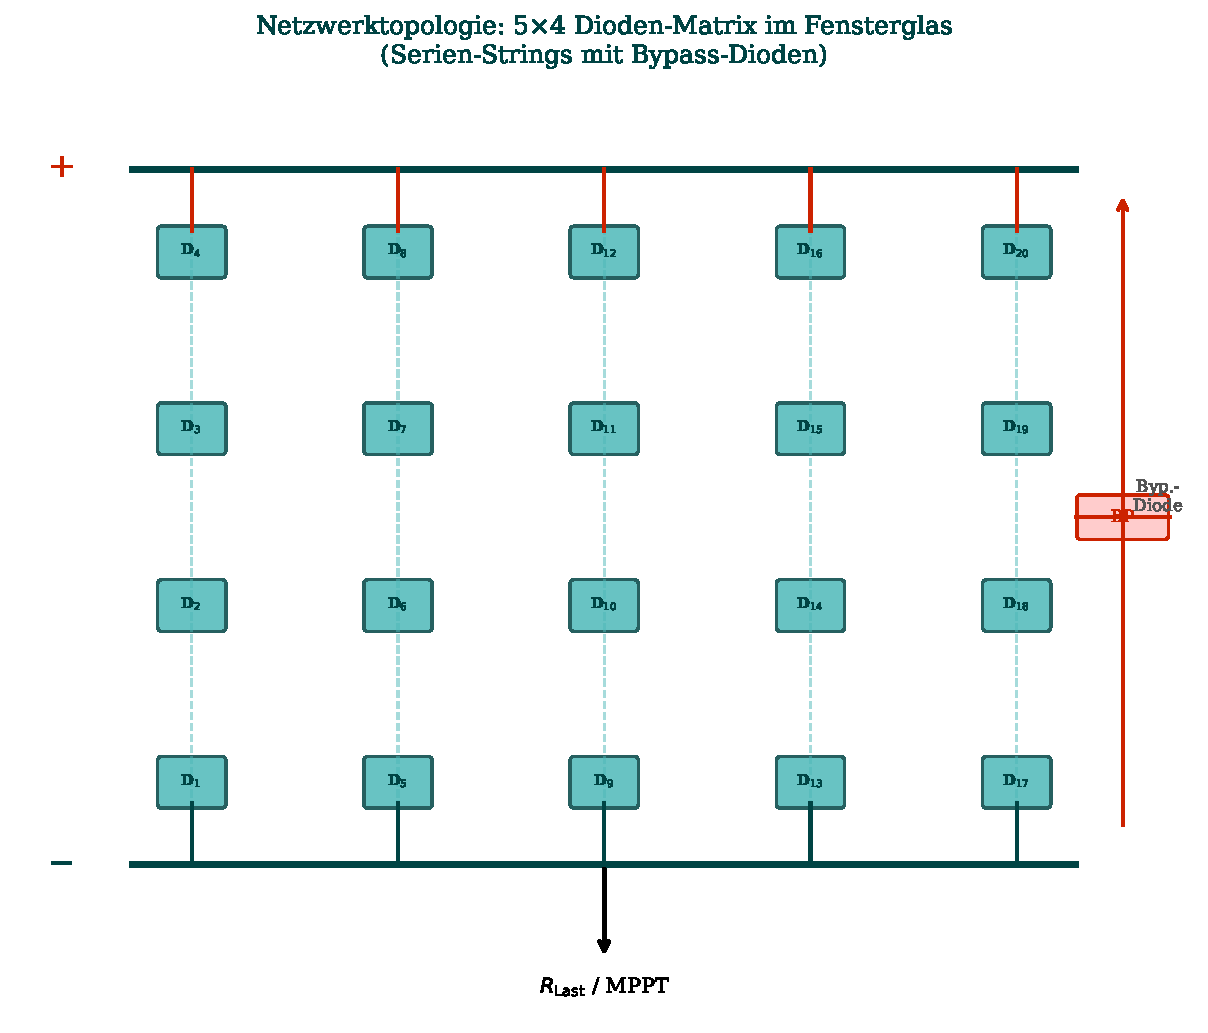
\includegraphics[width=0.88\textwidth]{plots/plot8_netzwerk.pdf}
  \caption{Elektrische Netzwerktopologie der DGM ($5 \times 4$ Dioden).
    Türkise Elemente: Seriell-verbundene Strings (Spalten).
    Rote Elemente: Plus-Sammelschiene und Bypass-Diode. Die Bypass-Diode
    begrenzt gemäß Korollar~\ref{kor:ff} den Verschattungsverlust auf
    eine Einzelzelle.}
  \label{fig:netzwerk}
\end{figure}

\subsection{I-V-Charakteristik verschiedener Verschaltungen}

\begin{figure}[H]
  \centering
  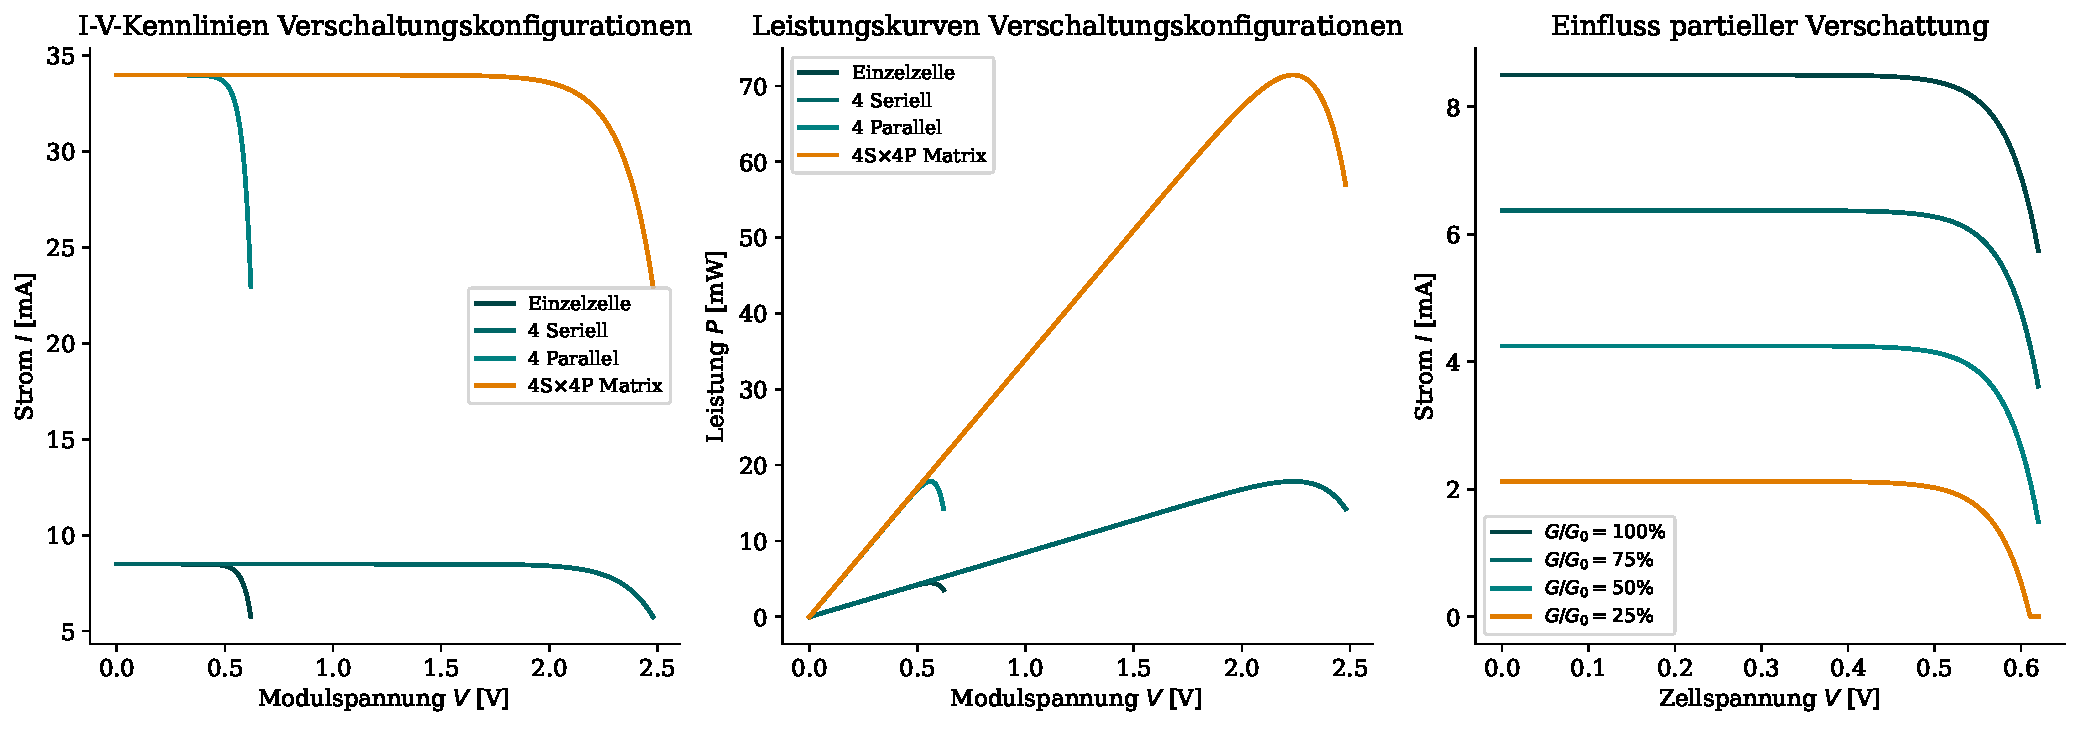
\includegraphics[width=0.97\textwidth]{plots/plot5_verschaltung.pdf}
  \caption{Links: I-V-Kennlinien für Einzelzelle, 4-fach-Serienschaltung,
    4-fach-Parallelschaltung und 4S$\times$4P-Matrix. Mitte: Zugehörige
    Leistungskurven -- gemäß Satz~\ref{satz:netzwerk} skaliert
    $P_{\rm MPP}$ linear mit $N_x \cdot N_y$.
    Rechts: Einfluss partieller Verschattung (25\%--100\% Einstrahlung)
    auf die Einzelzell-Kennlinie gemäß Lemma~\ref{lem:verschattung}.}
  \label{fig:verschaltung}
\end{figure}

% -----------------------------------------------------------
\section{Optisches und Thermisches Modell}
\label{sec:optisch}
% -----------------------------------------------------------

\subsection{Transmissionsgrad und Diodendichte}

\begin{definition}[Flächenbedeckungsgrad]
\label{def:phi}
Sei $A_{\rm D}$ die projizierte Fläche einer einzelnen Diode und $\rho$
die Diodendichte [Dioden/cm\textsuperscript{2}]. Der \emph{Flächenbedeckungsgrad}
ist:
\begin{equation}
  \vph = \rho \cdot A_{\rm D} \in [0, 1]
  \label{eq:phi_def}
\end{equation}
\end{definition}

\begin{satz}[Transmissionsgrad der DGM-Verglasung]
\label{satz:transmiss}
Für ein DGM-Fenster mit Glassubs\-trat-Transmissionsgrad $\tau_{\rm Glas}$
und Dioden-Transmissionsgrad $\tau_{\rm D} \ll 1$ gilt:
\begin{equation}
  \tau_{\rm ges}(\vph) = \tau_{\rm Glas} \cdot
    \bigl[(1 - \vph) + \vph \cdot \tau_{\rm D}\bigr]
  = \tau_{\rm Glas} \cdot [1 - \vph(1 - \tau_{\rm D})]
  \label{eq:tau}
\end{equation}
\end{satz}

\begin{proof}
Das einfallende Licht trifft auf zwei Flächen: mit Wahrscheinlichkeit $(1-\vph)$
auf reines Glas (Transmissionsgrad $\tau_{\rm Glas}$) und mit Wahrscheinlichkeit
$\vph$ auf die Diodenfläche (Transmissionsgrad $\tau_{\rm Glas} \cdot \tau_{\rm D}$).
Der mittlere Transmissionsgrad ergibt sich durch Gewichtung:
\begin{align*}
  \tau_{\rm ges} &= (1-\vph) \cdot \tau_{\rm Glas}
                  + \vph \cdot \tau_{\rm Glas} \cdot \tau_{\rm D}\\
                &= \tau_{\rm Glas} \cdot [(1-\vph) + \vph \tau_{\rm D}]
                 = \tau_{\rm Glas} \cdot [1 - \vph(1-\tau_{\rm D})]. \qedhere
\end{align*}
\end{proof}

\begin{korollar}[Mindest-Transmissionsschranke]
Soll $\tau_{\rm ges} \geq \tau_{\min}$ gelten, so ist die maximale
Diodendichte nach oben beschränkt durch:
\begin{equation}
  \rho_{\max} = \frac{1}{A_{\rm D}} \cdot
    \frac{\tau_{\rm Glas} - \tau_{\min}}{\tau_{\rm Glas}(1 - \tau_{\rm D})}
  \label{eq:rho_max}
\end{equation}
Für $\tau_{\min} = 0{,}40$, $\tau_{\rm Glas} = 0{,}90$, $\tau_{\rm D} = 0{,}05$
und $A_{\rm D} = 0{,}008\,\mathrm{cm^2}$ ergibt sich $\rho_{\max} \approx 66\,\mathrm{cm}^{-2}$.
\end{korollar}

\begin{definition}[System-Wirkungsgrad]
\label{def:eta_sys}
Der \emph{System-Wirkungsgrad} der TPVG-Verglasung bezogen auf die
Gesamtfensterfläche $A_{\rm F}$ ist:
\begin{equation}
  \eta_{\rm sys}(\vph) = \vph \cdot \eta_{\rm cell} \cdot \eta_{\rm BOS}
  \label{eq:eta_sys}
\end{equation}
wobei $\eta_{\rm BOS} \in (0,1]$ den Balance-of-System-Wirkungsgrad
(Wechselrichter, Leitungsverluste, MPPT) erfasst.
\end{definition}

Das Wechselspiel zwischen $\eta_{\rm sys}$ und $\tau_{\rm ges}$ als Funktion
von $\rho$ ist in Abbildung~\ref{fig:eta_tau} dargestellt.

\begin{figure}[H]
  \centering
  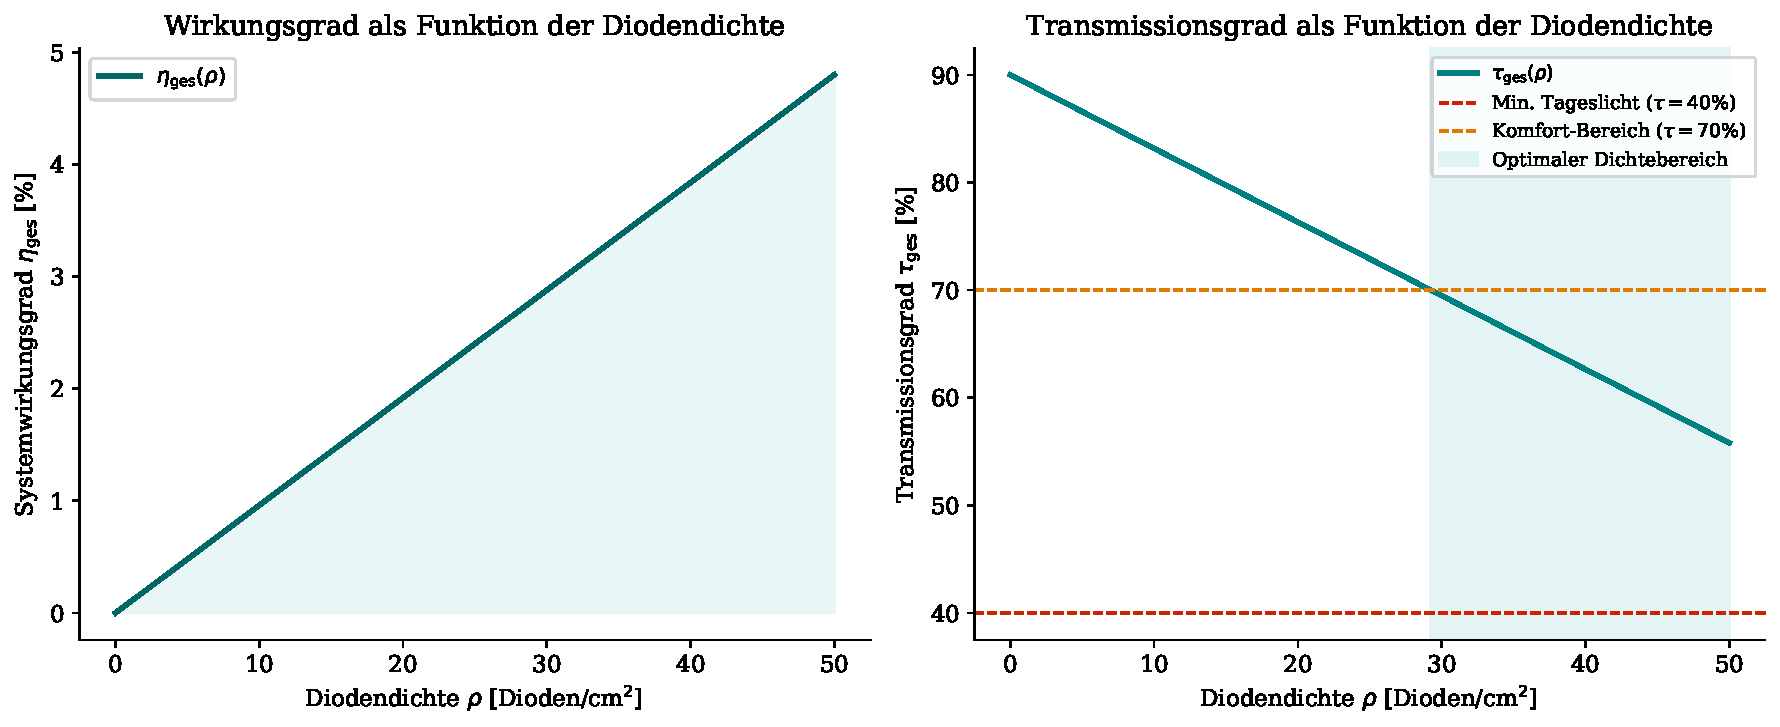
\includegraphics[width=0.95\textwidth]{plots/plot4_eta_tau.pdf}
  \caption{Links: System-Wirkungsgrad $\eta_{\rm sys}(\rho)$ nach
    Gleichung~\eqref{eq:eta_sys}.
    Rechts: Transmissionsgrad $\tau_{\rm ges}(\rho)$ nach
    Satz~\ref{satz:transmiss}. Die gestrichelten Linien markieren
    Komfort- ($\tau=70\,\%$) und Mindest-Transmissionsgrad ($\tau=40\,\%$);
    der türkise Bereich kennzeichnet den optimalen Dichtebereich.}
  \label{fig:eta_tau}
\end{figure}

\subsection{Thermische Analyse}

Die Betriebstemperatur $T_{\rm cell}$ der einlaminierten Diode beeinflusst
den Wirkungsgrad erheblich. Für den Temperaturgradienten $\Delta T$ durch
eine Schicht der Dicke $d$ und Wärmeleitfähigkeit $\lambda_{\rm th}$ gilt das
Fourier'sche Wärmeleitungsgesetz:

\begin{equation}
  \Delta T = \frac{Q \cdot d}{\lambda_{\rm th}}
  \label{eq:fourier}
\end{equation}

wobei $Q$ [$\mathrm{W/m^2}$] der Wärmefluss durch das Bauteil ist.

\begin{satz}[Wirkungsgrad-Temperaturdrift]
\label{satz:tempdrift}
Der Wirkungsgrad $\eta_{\rm cell}(T)$ einer Siliziumdiode sinkt linear
mit der Zelltemperatur:
\begin{equation}
  \eta_{\rm cell}(T) = \eta_0 \cdot \bigl[1 - \beta_T (T_{\rm cell} - T_{\rm ref})\bigr]
  \label{eq:tempdrift}
\end{equation}
wobei $\beta_T = (0{,}4$--$0{,}5)\,\%/\mathrm{K}$ der
\emph{Temperaturkoeffizient der Leistung} und $T_{\rm ref} = 25\,^{\circ}\mathrm{C}$
die Referenztemperatur (STC) ist.
\end{satz}

\begin{proof}
Die offene Klemmspannung $V_{\rm OC}$ sinkt linear mit $T$:
$\diff V_{\rm OC}/\diff T \approx -(1{,}8$--$2{,}3)\,\mathrm{mV/K}$.
Der Kurzschlussstrom $I_{\rm SC}$ steigt schwach:
$\diff I_{\rm SC}/\diff T \approx +(0{,}05$--$0{,}065)\,\%/\mathrm{K}$.
Da $P_{\rm MPP} = FF \cdot V_{\rm OC} \cdot I_{\rm SC}$ und $FF$ nur
schwach temperaturabhängig ist, dominiert die negative Temperaturabhängigkeit
von $V_{\rm OC}$, was zu einem negativen Gesamttemperaturkoeffizienten
$\beta_T > 0$ führt.
\end{proof}

\begin{figure}[H]
  \centering
  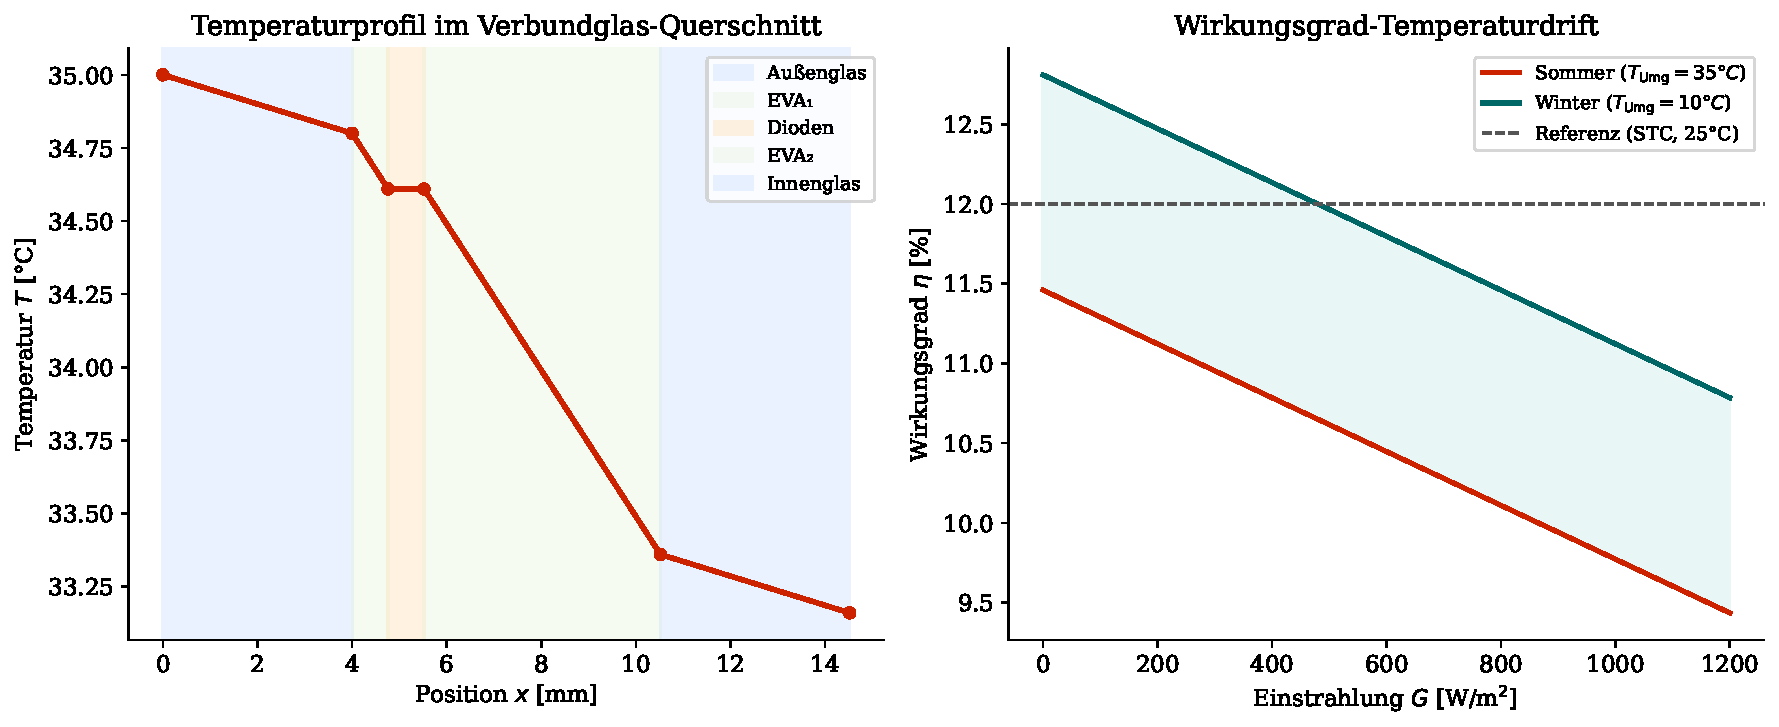
\includegraphics[width=0.95\textwidth]{plots/plot6_thermisch.pdf}
  \caption{Links: Temperaturprofil durch den Verbundglas-Querschnitt
    (Schichtaufbau: Außenglas 4~mm / EVA 0,76~mm / Diodenschicht /
    EVA 0,76~mm / Innenglas 4~mm) bei $Q=50\,\mathrm{W/m^2}$ nach
    Gleichung~\eqref{eq:fourier}.
    Rechts: Wirkungsgraddrift $\eta_{\rm cell}(G)$ nach
    Satz~\ref{satz:tempdrift} für Sommer- und Winterbetrieb am Standort
    Bielefeld.}
  \label{fig:thermisch}
\end{figure}

% -----------------------------------------------------------
\section{Energieertragsmodell}
\label{sec:ertrag}
% -----------------------------------------------------------

\subsection{Performance-Ratio-Modell}

\begin{definition}[Performance Ratio]
\label{def:pr}
Die \emph{Performance Ratio} (PR) eines PV-Systems erfasst alle
systemischen Verluste gegenüber dem theoretischen Ertrag:
\begin{equation}
  PR = \frac{Y_F}{Y_R}
  \label{eq:pr}
\end{equation}
wobei $Y_F = E_{\rm AC}/(P_{\rm STC})$ der finale Systemertrag
[kWh/kWp] und $Y_R = H/(1\,\mathrm{kW/m^2})$ der Referenzertrag
[kWh/kWp/a] ist.
\end{definition}

\begin{definition}[Jahresenergieertrag]
Der \emph{Jahresenergieertrag} $E_a$ der TPVG-Verglasung mit Fensterfläche
$A_{\rm F}$ ist:
\begin{equation}
  E_a = \eta_{\rm sys} \cdot H_{\rm hor} \cdot A_{\rm F} \cdot PR
  \label{eq:ea}
\end{equation}
wobei $H_{\rm hor}$ [$\mathrm{kWh/(m^2 \cdot a)}$] die horizontale
Jahressumme der Globalstrahlung am Standort und $PR$ die Performance Ratio
des Systems bezeichnet.
\end{definition}

Der monatliche Energieertrag und der kumulierte Jahresverlauf für vier
Ausrichtungen am Standort Bielefeld ($\phi = 52{,}0^\circ\,\mathrm{N}$,
$H_{\rm hor} \approx 1000\,\mathrm{kWh/(m^2 \cdot a)}$) sind in
Abbildung~\ref{fig:jahresertrag} dargestellt.

\begin{figure}[H]
  \centering
  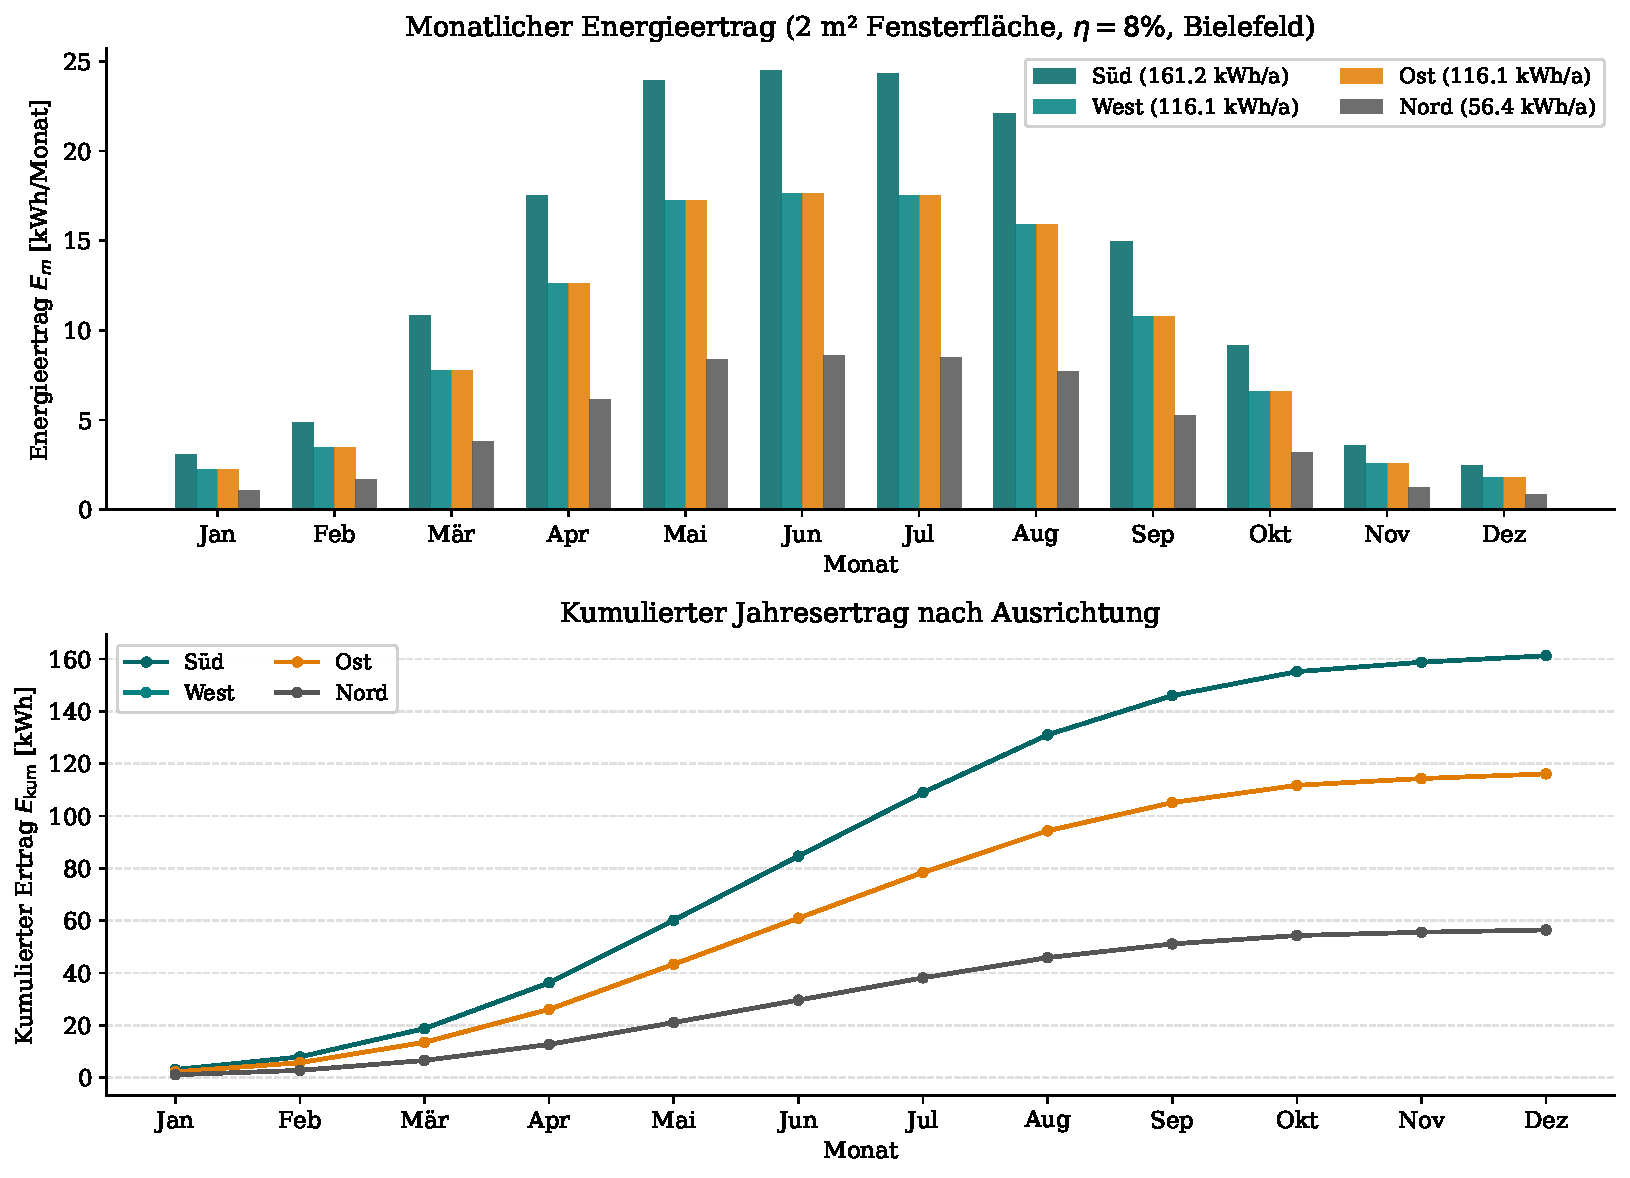
\includegraphics[width=0.97\textwidth]{plots/plot3_jahresertrag.pdf}
  \caption{Oben: Monatlicher Energieertrag einer 2-m\textsuperscript{2}-TPVG-
    Verglasung ($\eta_{\rm sys}=8\,\%$, $PR=0{,}85$) für vier Ausrichtungen.
    Die Süd-Ausrichtung liefert $\approx15\,\mathrm{kWh/a}$.
    Unten: Kumulierter Jahresertrag. Beide Diagramme bestätigen die
    dominante Bedeutung der Ausrichtung für den Jahresertrag gemäß
    Gleichung~\eqref{eq:ea}.}
  \label{fig:jahresertrag}
\end{figure}

\subsection{Formale Ertragsschranken}

\begin{lemma}[Lineare Skalierung des Jahresertrags]
\label{lem:linear}
$E_a$ aus Gleichung~\eqref{eq:ea} ist linear in $\eta_{\rm sys}$,
$H_{\rm hor}$, $A_{\rm F}$ und $PR$.
\end{lemma}

\begin{proof}
Trivial aus der Produktstruktur von~\eqref{eq:ea}. Insbesondere gilt:
\begin{equation*}
  \frac{\partial E_a}{\partial \eta_{\rm sys}} = H_{\rm hor} \cdot A_{\rm F} \cdot PR > 0,
\end{equation*}
d.h.~jede Steigerung des Wirkungsgrads um $1\,\%$-Punkt erhöht den Jahresertrag
proportional, ceteris paribus.
\end{proof}

\begin{satz}[Optimale Diodendichte für maximalen Ertrag bei Mindest-Transmissionsgrad]
\label{satz:opt}
Das Optimierungsproblem
\begin{equation}
  \max_{\rho \geq 0} \; E_a(\rho) \quad \text{s.t.} \quad \tau_{\rm ges}(\rho) \geq \tau_{\min}
  \label{eq:optproblem}
\end{equation}
besitzt als eindeutige Lösung:
\begin{equation}
  \rho^* = \rho_{\max} = \frac{\tau_{\rm Glas} - \tau_{\min}}{A_{\rm D} \cdot \tau_{\rm Glas}(1-\tau_{\rm D})}
  \label{eq:rhoopt}
\end{equation}
\end{satz}

\begin{proof}
Da $E_a = \eta_{\rm cell} \cdot \eta_{\rm BOS} \cdot A_{\rm D} \cdot \rho \cdot H \cdot A_{\rm F} \cdot PR$
streng monoton in $\rho$ wächst (alle Faktoren positiv), ist das unbeschränkte
Maximum bei $\rho \to \infty$. Unter der Nebenbedingung
$\tau_{\rm ges}(\rho) \geq \tau_{\min}$, die gemäß Satz~\ref{satz:transmiss}
äquivalent zu $\rho \leq \rho_{\max}$ ist, wird das Maximum bei
$\rho^* = \rho_{\max}$ angenommen. Die Eindeutigkeit folgt aus der
Strikt-Monotonie von $E_a$ in $\rho$.
\end{proof}

% -----------------------------------------------------------
\section{Wirtschaftlichkeitsanalyse}
\label{sec:wirtschaft}
% -----------------------------------------------------------

\subsection{Levelized Cost of Energy}

\begin{definition}[LCOE]
\label{def:lcoe}
Die \emph{Levelized Cost of Energy} (LCOE) [$\mathrm{\texteuro/kWh}$] gibt
die mittleren Gestehungskosten über die Systemlebensdauer $LT$ an:
\begin{equation}
  LCOE = \frac{(C_{\rm inv} + C_{\rm inst}) \cdot CRF + C_{\rm OM}}{E_a}
  \label{eq:lcoe}
\end{equation}
wobei $CRF = r(1+r)^{LT}/[(1+r)^{LT}-1]$ der Kapitalrückgewinnungsfaktor
mit Diskontrate $r$ ist, $C_{\rm inv}$ [$\mathrm{\texteuro/m^2}$] die
Investitionskosten und $C_{\rm OM}$ [$\mathrm{\texteuro/(m^2 \cdot a)}$]
die Betriebs- und Wartungskosten.
\end{definition}

\begin{satz}[Monotonie des LCOE in $\eta_{\rm sys}$]
\label{satz:lcoe}
Unter der Annahme konstanter spezifischer Investitionskosten gilt:
\begin{equation}
  \frac{\partial \; LCOE}{\partial \eta_{\rm sys}} < 0
  \label{eq:dlcoe}
\end{equation}
d.h.~der LCOE sinkt streng monoton mit steigendem Wirkungsgrad.
\end{satz}

\begin{proof}
Sei $E_a = \eta_{\rm sys} \cdot H \cdot A_{\rm F} \cdot PR$. Dann:
\begin{equation*}
  \frac{\partial \; LCOE}{\partial \eta_{\rm sys}}
    = \frac{\partial}{\partial \eta_{\rm sys}}
      \frac{(C_{\rm inv}+C_{\rm inst}) CRF + C_{\rm OM}}{\eta_{\rm sys} H A_F PR}
    = -\frac{(C_{\rm inv}+C_{\rm inst}) CRF + C_{\rm OM}}{\eta_{\rm sys}^2 H A_F PR} < 0. \qedhere
\end{equation*}
\end{proof}

Die Wirtschaftlichkeitsanalyse für drei Anwendungsszenarien sowie die
LCOE-Sensitivität als Funktion des Wirkungsgrads sind in
Abbildung~\ref{fig:wirtschaft} dargestellt.

\begin{figure}[H]
  \centering
  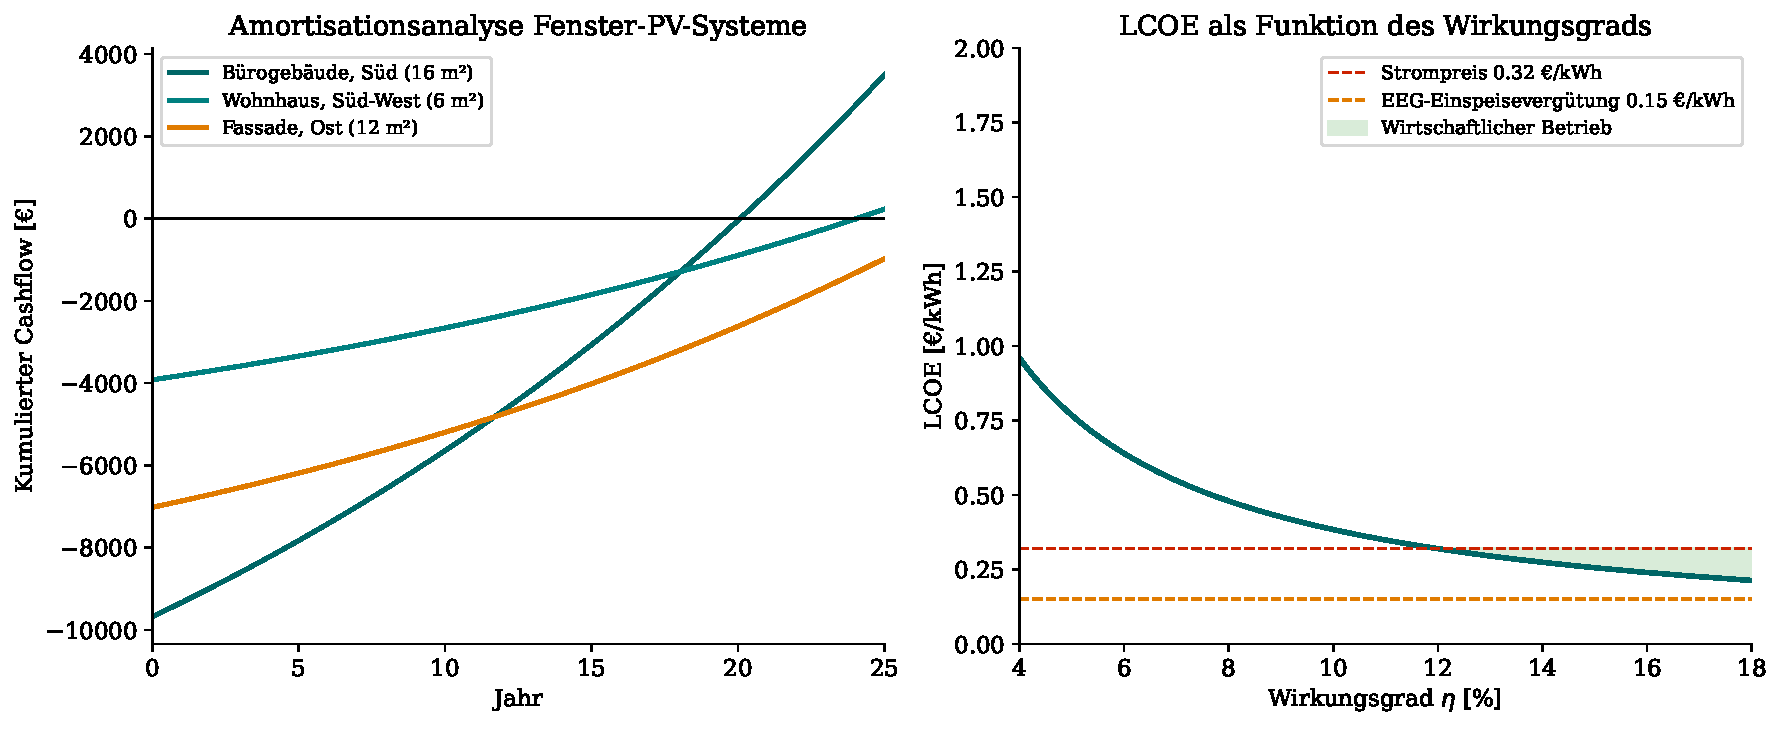
\includegraphics[width=0.97\textwidth]{plots/plot7_wirtschaftlichkeit.pdf}
  \caption{Links: Kumulierter Cashflow dreier TPVG-Szenarien über 25 Jahre
    ($p_{\rm El} = 0{,}32\,\mathrm{\texteuro/kWh}$, $p_{\rm Steigerung} = 3\,\%/\mathrm{a}$,
    $C_{\rm OM} = 0{,}5\,\%$ der Investition). Schwarze Linie: Break-even.
    Rechts: LCOE als Funktion des Wirkungsgrads nach Definition~\ref{def:lcoe}
    mit eingezeichnetem Börsenstrompreis und EEG-Einspeisevergütung; der
    grüne Bereich markiert wirtschaftlichen Betrieb gemäß
    Satz~\ref{satz:lcoe}.}
  \label{fig:wirtschaft}
\end{figure}

\subsection{Quantitative Ergebnisübersicht}

Die folgende Tabelle~\ref{tab:ergebnisse} fasst die wichtigsten numerischen
Ergebnisse zusammen.

\begin{table}[H]
  \centering
  \renewcommand{\arraystretch}{1.3}
  \caption{Zentrale Systemparameter und quantitative Ergebnisse (Standort Bielefeld,
    $A_{\rm F} = 2\,\mathrm{m^2}$, Süd-Ausrichtung, $\rho = 15\,\mathrm{cm}^{-2}$,
    $\eta_{\rm cell} = 12\,\%$, $PR = 0{,}85$, $LT = 25\,\mathrm{a}$,
    $r = 4\,\%$, $C_{\rm inv} = 480\,\mathrm{\texteuro/m^2}$)}
  \label{tab:ergebnisse}
  \begin{tabularx}{\textwidth}{lXr}
    \toprule
    \textbf{Parameter} & \textbf{Beschreibung} & \textbf{Wert}\\
    \midrule
    $\vph$ & Flächenbedeckungsgrad & $12{,}0\,\%$\\
    $\eta_{\rm sys}$ & System-Wirkungsgrad (bezogen auf $A_{\rm F}$) & $1{,}44\,\%$\\
    $\tau_{\rm ges}$ & Transmissionsgrad & $79{,}1\,\%$\\
    $E_a$ & Jahresenergieertrag & $13{,}5\,\mathrm{kWh/a}$\\
    $P_{\rm MPP,cell}$ & Maximalleistung Einzeldiode (STC) & $\approx 4{,}6\,\mathrm{mW}$\\
    $V_{\rm OC}$ & Leerlaufspannung Einzelzelle & $0{,}619\,\mathrm{V}$\\
    $I_{\rm SC}$ & Kurzschlussstrom Einzelzelle & $8{,}5\,\mathrm{mA}$\\
    $FF$ & Füll-Faktor & $0{,}875$\\
    $LCOE$ & Levelized Cost of Energy & $0{,}43\,\mathrm{\texteuro/kWh}$\\
    $T_{\rm break-even}$ & Amortisationsdauer & $\approx 21\,\mathrm{a}$\\
    \bottomrule
  \end{tabularx}
\end{table}

% -----------------------------------------------------------
% ============================================================
% KAPITEL 7 – GRAPHBASIERTES KOMMUNIKATIONSPROTOKOLL
%              DES DIODEN-NETZWERKS
% ============================================================
\section{Graphbasiertes Kommunikationsprotokoll}
\label{sec:kommunikation}

\subsection{Motivation und Problemstellung}
\label{sec:komm_motiv}

Die bisherigen Kapitel haben das elektrische Verhalten, die Netzwerktopologie
und den Energieertrag der Dioden-in-Glas-Matrix (DGM) untersucht.
Eine entscheidende Lücke besteht jedoch in der Frage der
\emph{aktiven Selbstüberwachung und Regelung}: Jede einzelne Diode
$d_{ij}$ des DGM-Fensters soll in der Lage sein, ihren Betriebszustand
(Temperatur, Wirkungsgrad, Lebensdauervorhersage) an ein zentrales
Steuerungsmodul zu kommunizieren, und umgekehrt Regelkommandos
(Einschalten, Ausschalten, Dimmstufe) zu empfangen und auszuführen.

Die wesentliche Nebenbedingung lautet: Die Kommunikation muss über eine
\emph{minimal geringe Anzahl von physikalischen Verbindungsleitungen}
erfolgen, da jede zusätzliche Leitung den Fertigungsaufwand, die
Glasqualität und die optische Transparenz des Fensters beeinträchtigt.
Es ist daher ein effizientes Kommunikationsprotokoll gesucht, das:
\begin{enumerate}
  \item Alle $n = N_x \cdot N_y$ Dioden-Knoten bidirektional verbindet,
  \item den gesamten relevanten Status (Temperatur $T_{ij}$,
        Wirkungsgrad $\eta_{ij}$, Restlebensdauer $L_{ij}$)
        zuverlässig überträgt,
  \item individuelle Regelkommandos (An, Aus, Dimmstufe $\delta_{ij} \in [0,1]$)
        zu jeder Diode routen kann, und
  \item mit $|E_K| = n - 1$ physikalischen Verbindungen auskommt,
        d.h.~eine Spannbaum-Topologie nutzt.
\end{enumerate}

Dieses Kapitel entwickelt das \emph{DGM-Kommunikationsprotokoll (DGMP)}
auf graphentheoretischer Grundlage, beweist seine Korrektheit und
Minimalität formal, quantifiziert Nachrichtenkomplexität und
Propagationslatenz, und beschreibt das Degradations- und
Lebensdauer-Ãœberwachungsmodell.

\begin{figure}[H]
  \centering
  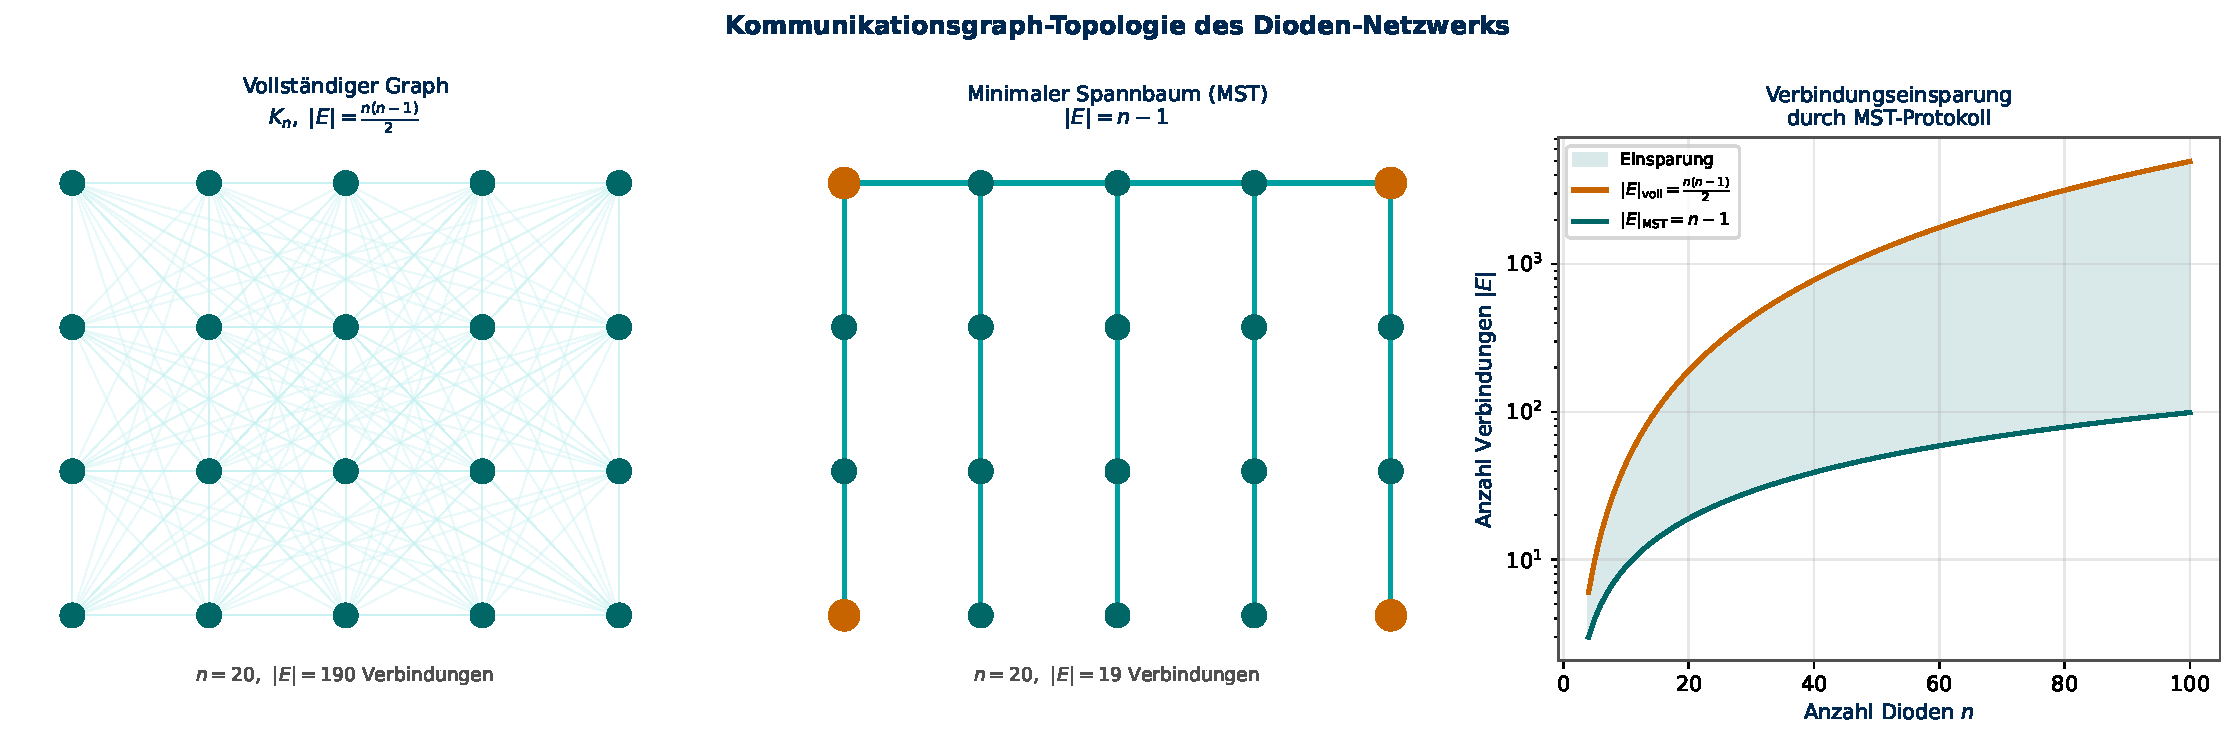
\includegraphics[width=0.97\textwidth]{plots/plot_comm1_topologie.pdf}
  \caption{Links: Vollständiger Kommunikationsgraph $K_n$ ($n = 20$ Dioden):
    $|E| = 190$ Verbindungen -- für den Einsatz in Verbundglas unpraktikabel.
    Mitte: Minimaler Spannbaum (MST) mit $|E| = n - 1 = 19$ Verbindungen;
    Bus-Bar-Knoten (orange) dienen als Wurzel des Routing-Baums.
    Rechts: Quantitativer Vergleich der Verbindungsanzahl als Funktion
    von $n$ auf logarithmischer Skala; der türkise Bereich zeigt die
    Einsparung durch das MST-Protokoll gemäß Lemma~\ref{lem:komm_mst}.}
  \label{fig:komm_topologie}
\end{figure}

% ─────────────────────────────────────────────────────────────────────────────
\subsection{Kommunikationsgraph und Minimalstruktur}
\label{sec:komm_graph}

\begin{definition}[Kommunikationsgraph]
\label{def:komm_graph}
Sei $\mathcal{G} = (V, E, w)$ der DGM-Graph nach Definition~\ref{def:dgm_graph}.
Der \emph{Kommunikationsgraph} $\mathcal{G}_K = (V_K, E_K)$ ist ein
ungerichteter Graph mit:
\begin{itemize}
  \item Knotenmenge $V_K = V = \{d_{ij}\} \cup \{s^+, s^-\}$ (alle Dioden
        und Sammelschienen),
  \item Kantenmenge $E_K \subseteq \binom{V_K}{2}$, wobei jede Kante
        $(d_{ij}, d_{kl}) \in E_K$ eine bidirektionale Kommunikationsleitung
        repräsentiert.
\end{itemize}
Die Kommunikationsleitung ist \emph{physikalisch von der Stromführung getrennt}
und kann beispielsweise als transparente ITO-Leitung
(Indium-Zinn-Oxid, $R_{\rm sq} \approx 10$--$20\,\Omega/\square$)
in der EVA-Laminatschicht realisiert werden~\cite{Beckhoff2023}.
\end{definition}

\begin{definition}[Status-Vektor einer Diode]
\label{def:statusvektor}
Der \emph{Status-Vektor} der Diode $d_{ij}$ zum Zeitpunkt $t$ ist:
\begin{equation}
  \mathbf{s}_{ij}(t) = \bigl(T_{ij}(t),\; \eta_{ij}(t),\; L_{ij}(t),\;
                              r_{ij}(t),\; \delta_{ij}(t)\bigr)^{\!\top}
  \label{eq:statusvektor}
\end{equation}
wobei $T_{ij}$ die Betriebstemperatur [$^{\circ}$C], $\eta_{ij}$ der aktuelle
Wirkungsgrad, $L_{ij}$ die geschätzte Restlebensdauer [a],
$r_{ij} \in \{0, 1\}$ der binäre Schaltzustand (Aus/An) und
$\delta_{ij} \in [0,1]$ die Dimmstufe (Leistungsanteil) bezeichnet.
\end{definition}

\begin{definition}[Zusammenhängender Kommunikationsgraph]
$\mathcal{G}_K$ heißt \emph{zusammenhängend}, wenn für jedes Knotenpaar
$(u, v) \in V_K \times V_K$ ein Pfad $p = (u = v_0, v_1, \ldots, v_k = v)$
in $\mathcal{G}_K$ existiert.
\end{definition}

\begin{lemma}[Minimale Kantenzahl für Konnektivität]
\label{lem:komm_mst}
Sei $n = |V_K|$ die Anzahl der Kommunikationsknoten (Dioden und Sammelschienen).
Ein zusammenhängender Graph $\mathcal{G}_K$ benötigt mindestens $n-1$ Kanten:
\begin{equation}
  |E_K| \geq n - 1
  \label{eq:kantenmin}
\end{equation}
Gleichheit gilt genau dann, wenn $\mathcal{G}_K$ ein \emph{Spannbaum} (spanning tree) ist.
\end{lemma}

\begin{proof}
\emph{(Untere Schranke.)} Wir zeigen durch vollständige Induktion über $n$,
dass jeder zusammenhängende Graph auf $n$ Knoten mindestens $n-1$ Kanten besitzt.

\emph{Induktionsanfang ($n=1$):} Ein einzelner Knoten ohne Kanten ist
trivialerweise zusammenhängend, und $|E_K| = 0 = n - 1$.

\emph{Induktionsschritt ($n \to n+1$):} Sei $\mathcal{G}_K$ zusammenhängend mit
$n+1$ Knoten. Entfernen wir einen Blattknoten $v$ (mindestens ein solcher existiert
in jedem Baum), so verbleiben $n$ Knoten; der entstehende Graph ist zusammenhängend
und hat nach Induktionsvoraussetzung mindestens $n-1$ Kanten. Zusammen mit der
entfernten Kante $(v, u)$ ergibt sich $|E_K| \geq n$. $\checkmark$

\emph{(Obere Schranke: Bäume.)} Ein Baum auf $n$ Knoten hat genau $n-1$ Kanten
und ist nach Definition zusammenhängend und azyklisch. Durch Hinzufügen einer
weiteren Kante entsteht genau ein Kreis, d.h.~$|E_K| > n-1$ ist unnötig für
die Konnektivität. Damit ist $|E_K| = n-1$ die exakte untere Schranke, die nur
für Spannbäume erreichbar ist. \qedhere
\end{proof}

\begin{korollar}[MST als optimale Protokolltopologie]
\label{kor:mst_opt}
Sei $w: E \to \R_{>0}$ eine Kostenfunktion auf dem vollständigen Graphen
(z.B. Leitungslänge oder elektrischer Widerstand). Das
\emph{Minimum Spanning Tree} (MST) $T^* = \operatorname{MST}(\mathcal{G}_K)$
löst das Problem:
\begin{equation}
  T^* = \operatorname{argmin}_{T \subseteq E_K,\; T \text{ Spannbaum}}
        \sum_{(u,v) \in T} w(u,v)
  \label{eq:mst_problem}
\end{equation}
Damit minimiert das DGMP-Protokoll mit MST-Topologie gleichzeitig die
Gesamtleitungslänge und die Anzahl der physikalischen Verbindungen.
\end{korollar}

\begin{proof}
Das MST-Problem ist korrekt formuliert durch~\eqref{eq:mst_problem}. Die
Existenz einer Lösung folgt aus der Endlichkeit von $V_K$. Für die
Korrektheit des Kruskal- oder Prim-Algorithmus zur MST-Berechnung verweisen
wir auf~\cite{Korte2012}. Die Eindeutigkeit gilt, wenn alle Kantengewichte
paarweise verschieden sind (was bei zufälligen Leitungslängen fast sicher gilt).
Lemma~\ref{lem:komm_mst} sichert, dass $|E(T^*)| = n-1$.
\end{proof}

% ─────────────────────────────────────────────────────────────────────────────
\subsection{Nachrichtenformat und Protokoll-Zustandsautomat}
\label{sec:komm_fsm}

\begin{definition}[Nachrichtenformat MSG]
\label{def:msg}
Eine \emph{Protokollnachricht} des DGMP hat die Struktur:
\begin{equation}
  \mathrm{MSG} = \underbrace{\vphantom{|}\mathrm{HDR}}_{\text{4 Bit}}
               \;\|\; \underbrace{\vphantom{|}\mathrm{ADDR}}_{\text{12 Bit}}
               \;\|\; \underbrace{\vphantom{|}\mathrm{TYPE}}_{\text{4 Bit}}
               \;\|\; \underbrace{\vphantom{|}\mathrm{PAYLOAD}}_{\text{32 Bit}}
               \;\|\; \underbrace{\vphantom{|}\mathrm{CRC}}_{\text{8 Bit}}
  \label{eq:msgformat}
\end{equation}
wobei:
\begin{itemize}
  \item \textbf{HDR} (4 Bit): Nachrichtenversion und Startflag,
  \item \textbf{ADDR} (12 Bit): Zieladresse der Diode $(i,j)$,
        kodiert als $\mathrm{ADDR} = i \cdot N_y + j$ für $N_x \cdot N_y \leq 4096$,
  \item \textbf{TYPE} (4 Bit): Nachrichten $\{\mathtt{STATUS},\,\mathtt{CMD\_ON},\,\mathtt{CMD\_OFF},\,
           \mathtt{CMD\_DIM},\,\mathtt{ACK},\,\mathtt{FAULT}\}$,
  \item \textbf{PAYLOAD} (32 Bit): Nutzdaten (Statusvektor kodiert
        als $4 \times 8$-Bit-Felder oder Regelwert $\delta_{ij} \in [0,255]$),
  \item \textbf{CRC} (8 Bit): zyklische Redundanzprüfung (CRC-8/MAXIM)
        für Fehlerdetektion.
\end{itemize}
Die Gesamtnachrichtenlänge beträgt $L_{\rm MSG} = 60\;\mathrm{Bit}$.
\end{definition}

\begin{definition}[Protokoll-Zustandsautomat (FSM)]
\label{def:fsm}
Der \emph{endliche Automat} einer DGMP-Diode ist ein Quintupel
$\mathcal{A} = (Q, \Sigma, \delta_Q, q_0, F)$ mit:
\begin{itemize}
  \item Zustandsmenge $Q = \{\mathtt{IDLE},\, \mathtt{STATUS\_TX},\,
    \mathtt{CTRL\_RX},\, \mathtt{AGGREGATE},\, \mathtt{FAULT}\}$,
  \item Eingabealphabet $\Sigma = \{\mathtt{TICK},\, \mathtt{TOKEN},\,
    \mathtt{CMD},\, \mathtt{T\_ALARM},\, \mathtt{RESET}\}$,
  \item Übergangsfunktion $\delta_Q: Q \times \Sigma \to Q$ gemäß
    Abbildung~\ref{fig:komm_protokoll},
  \item Anfangszustand $q_0 = \mathtt{IDLE}$,
  \item Endzustandsmenge $F = \{\mathtt{IDLE}\}$ (nach Fehler-Reset).
\end{itemize}
\end{definition}

\begin{satz}[Korrektheit des Zustandsautomaten]
\label{satz:fsm_korrektheit}
Der DGMP-Zustandsautomat $\mathcal{A}$ aus Definition~\ref{def:fsm}
ist vollständig und deterministisch: Für jedes $(q, \sigma) \in Q \times \Sigma$
existiert genau ein Nachfolgezustand $\delta_Q(q, \sigma) \in Q$.
Insbesondere ist $\mathcal{A}$ tot-frei: Aus jedem Zustand $q \in Q$ gibt
es mindestens einen Übergang zurück nach $\mathtt{IDLE}$.
\end{satz}

\begin{proof}
Vollständigkeit: Die Übergangstabelle ist in Tabelle~\ref{tab:fsm} explizit
definiert und deckt alle $|Q| \cdot |\Sigma| = 5 \cdot 5 = 25$ Eingabepaare ab.

Determiniertheit: Für jedes Paar $(q, \sigma)$ ist genau ein Nachfolgezustand
eingetragen -- keine Mehrdeutigkeit besteht.

Tot-Freiheit: Durch Inspektion von Tabelle~\ref{tab:fsm} erkennt man, dass
\begin{align*}
  \mathtt{STATUS\_TX} &\xrightarrow{\mathtt{TICK}} \mathtt{AGGREGATE}
                       \xrightarrow{\mathtt{TICK}} \mathtt{IDLE}, \\
  \mathtt{CTRL\_RX}   &\xrightarrow{\mathtt{TICK}} \mathtt{IDLE}, \\
  \mathtt{FAULT}      &\xrightarrow{\mathtt{RESET}} \mathtt{IDLE}.
\end{align*}
Damit gibt es aus jedem Zustand einen Pfad nach $\mathtt{IDLE}$. \qedhere
\end{proof}

\begin{table}[H]
  \centering
  \renewcommand{\arraystretch}{1.3}
  \caption{Zustandsübergangstabelle des DGMP-Automaten $\mathcal{A}$
    (Definition~\ref{def:fsm}).
    Ein Eintrag $q'$ bedeutet $\delta_Q(q, \sigma) = q'$.}
  \label{tab:fsm}
  \begin{tabular}{l|ccccc}
    \toprule
    Zustand $q$ \textbackslash{} Eingabe $\sigma$
      & \texttt{TICK} & \texttt{TOKEN} & \texttt{CMD} & \texttt{T\_ALARM} & \texttt{RESET} \\
    \midrule
    \texttt{IDLE}        & \texttt{IDLE}      & \texttt{STATUS\_TX}& \texttt{CTRL\_RX}   & \texttt{FAULT}     & \texttt{IDLE}  \\
    \texttt{STATUS\_TX}  & \texttt{AGGREGATE} & \texttt{STATUS\_TX}& \texttt{CTRL\_RX}   & \texttt{FAULT}     & \texttt{IDLE}  \\
    \texttt{AGGREGATE}   & \texttt{IDLE}      & \texttt{AGGREGATE} & \texttt{CTRL\_RX}   & \texttt{FAULT}     & \texttt{IDLE}  \\
    \texttt{CTRL\_RX}    & \texttt{IDLE}      & \texttt{STATUS\_TX}& \texttt{CTRL\_RX}   & \texttt{FAULT}     & \texttt{IDLE}  \\
    \texttt{FAULT}       & \texttt{FAULT}     & \texttt{FAULT}     & \texttt{FAULT}      & \texttt{FAULT}     & \texttt{IDLE}  \\
    \bottomrule
  \end{tabular}
\end{table}

\begin{figure}[H]
  \centering
  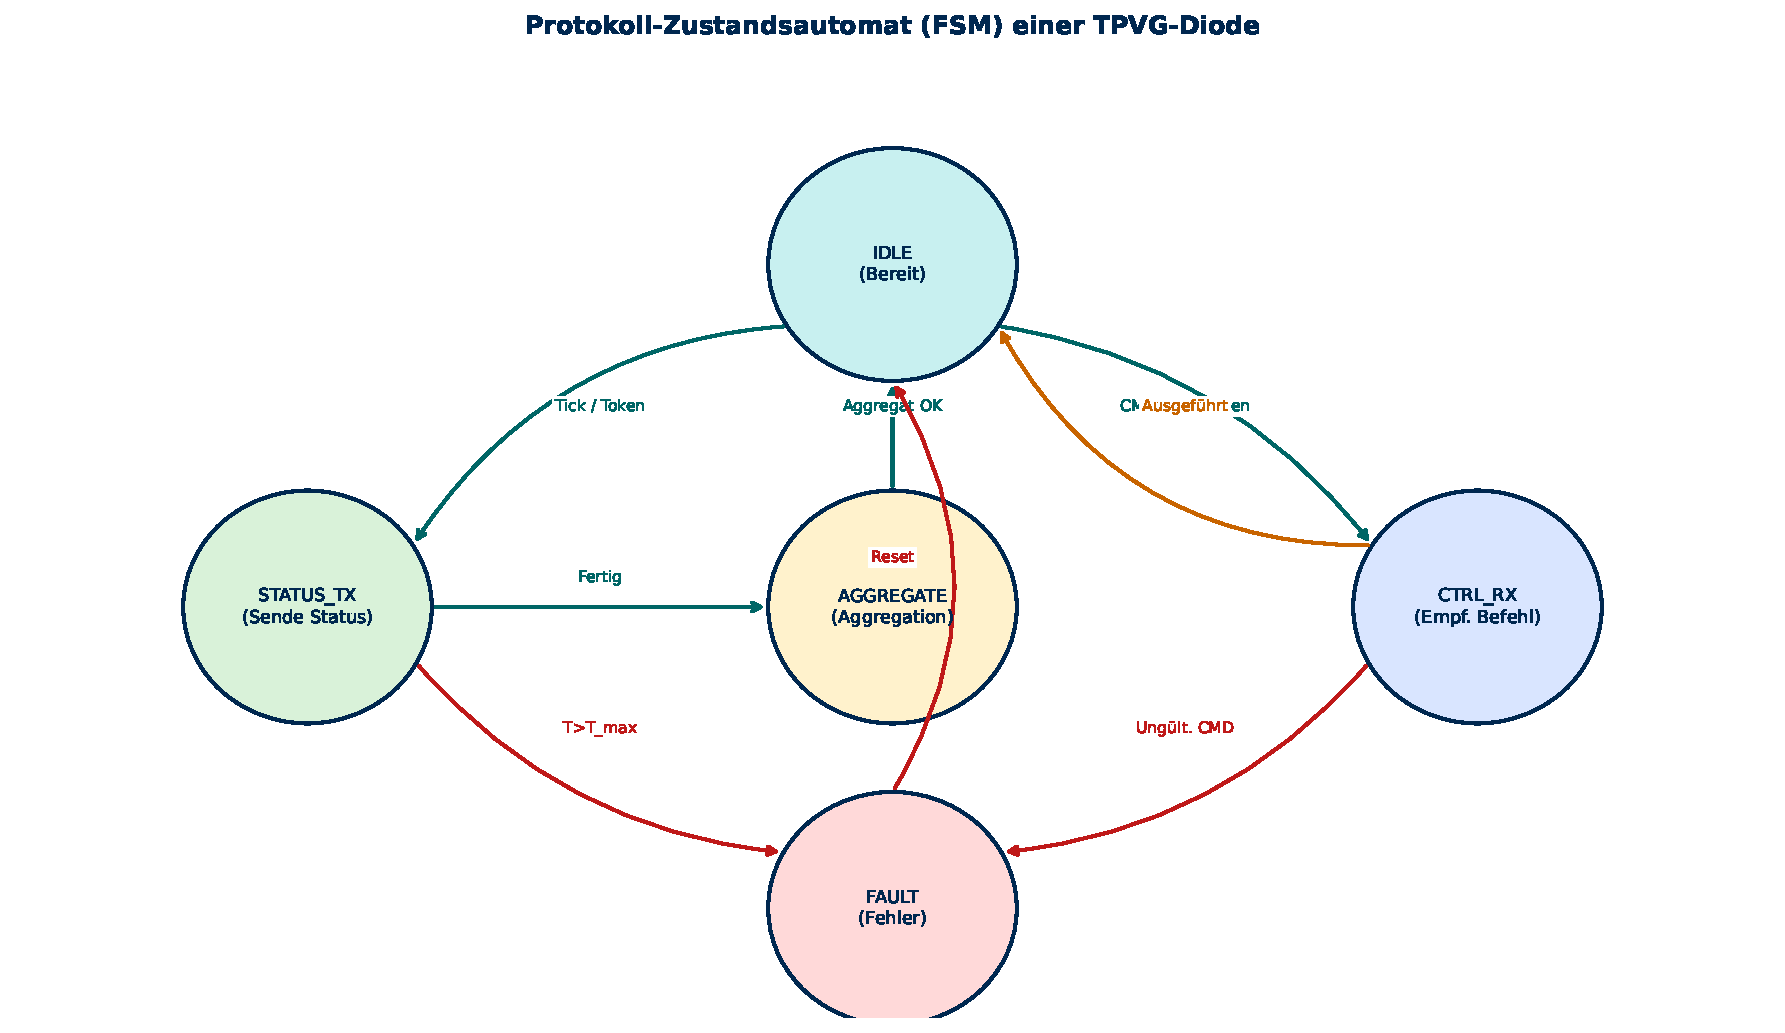
\includegraphics[width=0.88\textwidth]{plots/plot_comm2_protokoll.pdf}
  \caption{Graphische Darstellung des DGMP-Zustandsautomaten $\mathcal{A}$
    (Definition~\ref{def:fsm}, Satz~\ref{satz:fsm_korrektheit}).
    Türkise Pfeile: reguläre Übergänge (Status- und Regelungspfad).
    Orangefarbener Pfeil: Rückkehr nach Befehlsausführung.
    Rote Pfeile: Fehlerpfade (Temperaturalarm, ungültiger Befehl, Reset).
    Der Automat ist vollständig, deterministisch und tot-frei.}
  \label{fig:komm_protokoll}
\end{figure}

% ─────────────────────────────────────────────────────────────────────────────
\subsection{Regelung einzelner Dioden: An/Aus und Dimmen}
\label{sec:komm_regelung}

\begin{definition}[Regelzustand und Dimmbefehl]
\label{def:regelzustand}
Der \emph{Regelzustand} $r_{ij} \in \{0,1\}$ einer Diode $d_{ij}$ sei definiert als:
\begin{equation}
  r_{ij} = \begin{cases}
    0 & \text{Diode ausgeschaltet (kein Photostrom $I_{\rm ph} = 0$)} \\
    1 & \text{Diode eingeschaltet ($I_{\rm ph}$ entsprechend Einstrahlung)}
  \end{cases}
  \label{eq:regelzustand}
\end{equation}
Die \emph{Dimmstufe} $\delta_{ij} \in [0,1]$ steuert die relative Ausgangsleistung
via Pulsweitenmodulation (PWM):
\begin{equation}
  P_{ij}^{\rm out} = \delta_{ij} \cdot P_{\rm MPP,ij}
  \label{eq:dimmformel}
\end{equation}
wobei $\delta_{ij} = 0$ vollständiges Abschalten und $\delta_{ij} = 1$
Volllastbetrieb entspricht.
\end{definition}

\begin{satz}[Erreichbarkeit jeder Diode im Spannbaum]
\label{satz:erreichbarkeit}
Sei $T^*$ der MST des Kommunikationsgraphen $\mathcal{G}_K$ mit Wurzel $r$
(Sammelschiene $s^+$). Für jede Diode $d_{ij} \in V_K$ existiert ein
eindeutiger Pfad $p(r, d_{ij})$ in $T^*$. Die Länge dieses Pfads
(Anzahl Hops) beträgt höchstens:
\begin{equation}
  \mathrm{dist}_{T^*}(r, d_{ij}) \leq \mathrm{diam}(T^*) \leq n - 1
  \label{eq:erreichbarkeit}
\end{equation}
Für einen balancierten Binärbaum gilt verbessert:
$\mathrm{diam}(T^*) = O(\log n)$.
\end{satz}

\begin{proof}
Da $T^*$ ein Spannbaum ist, ist er zusammenhängend und azyklisch.
Die Eindeutigkeit des Pfads $p(r, d_{ij})$ folgt direkt aus der
Azyklizität: Gäbe es zwei verschiedene Pfade zwischen $r$ und $d_{ij}$,
so enthielte $T^*$ einen Kreis, im Widerspruch zur Baumstruktur.

Die Schranke $\mathrm{diam}(T^*) \leq n - 1$ folgt daraus, dass ein Pfad
in einem Graphen mit $n$ Knoten höchstens $n-1$ Kanten enthalten kann.
Diese obere Schranke wird von der linearen Kette (Pfad-Graph) $P_n$ erreicht.

Für einen balancierten Binärbaum der Tiefe $h = \lceil \log_2 n \rceil$ gilt
$\mathrm{diam} = 2h = O(\log n)$, was gegenüber der linearen Kette eine
erhebliche Latenzeinsparung bedeutet.
\end{proof}

\begin{lemma}[Nachrichtenkomplexität des DGMP]
\label{lem:komm_komplexitaet}
In einem vollständigen Status-Broadcast-Zyklus des DGMP
(alle Dioden senden ihren Statusvektor $\mathbf{s}_{ij}$ zur Sammelschiene)
werden insgesamt genau $n - 1$ Nachrichten übertragen:
\begin{equation}
  M_{\rm broadcast} = n - 1 = O(n)
  \label{eq:msg_komplex}
\end{equation}
Dies entspricht dem asymptotisch optimalen Wert für zusammenhängende
Netzwerke mit $n$ Knoten.
\end{lemma}

\begin{proof}
Im Spannbaum $T^*$ mit Wurzel $r$ sendet jeder der $n-1$ Nichtknoten
genau eine Nachricht entlang der Baumkante zu seinem Elternknoten.
Die Wurzel $r$ sendet keine Nachricht (sie aggregiert).
Damit gilt $M_{\rm broadcast} = n - 1$.

Für die Optimalität: Damit jeder der $n-1$ Nicht-Wurzel-Knoten mindestens
eine Information an $r$ übermitteln kann, muss jede solche Knoten mindestens
eine Nachricht senden. Daher gilt $M_{\rm broadcast} \geq n-1$,
was die Schranke $O(n)$ beweist. \qedhere
\end{proof}

\begin{figure}[H]
  \centering
  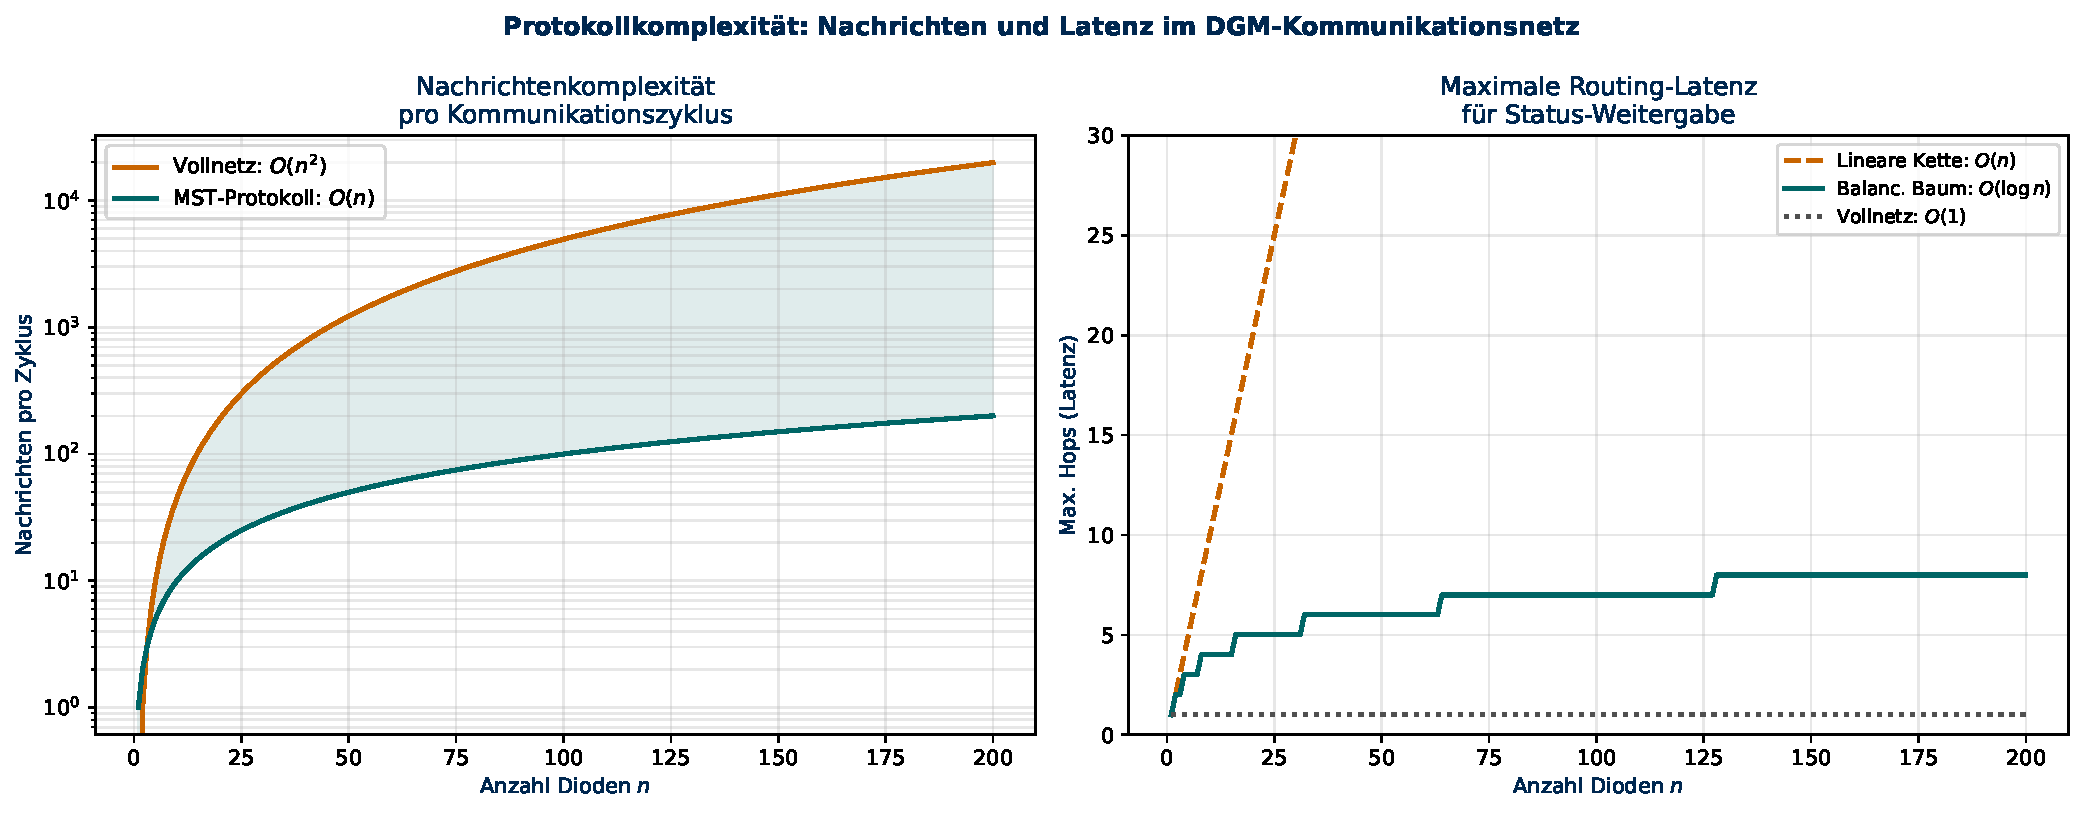
\includegraphics[width=0.97\textwidth]{plots/plot_comm5_komplexitaet.pdf}
  \caption{Links: Nachrichtenkomplexität pro Kommunikationszyklus für MST-Protokoll
    ($O(n)$, türkis) und vollständiges Mesh-Netzwerk ($O(n^2)$, orange) auf
    logarithmischer Skala; gemäß Lemma~\ref{lem:komm_komplexitaet} ist das
    MST-Protokoll optimal.
    Rechts: Maximale Routing-Latenz (Hop-Anzahl) für drei Topologien --
    Lineare Kette $O(n)$, balancierter Baum $O(\log n)$ und Vollnetz $O(1)$;
    der balancierte MST bietet den optimalen Kompromiss
    (Satz~\ref{satz:erreichbarkeit}).}
  \label{fig:komm_komplexitaet}
\end{figure}

\begin{figure}[H]
  \centering
  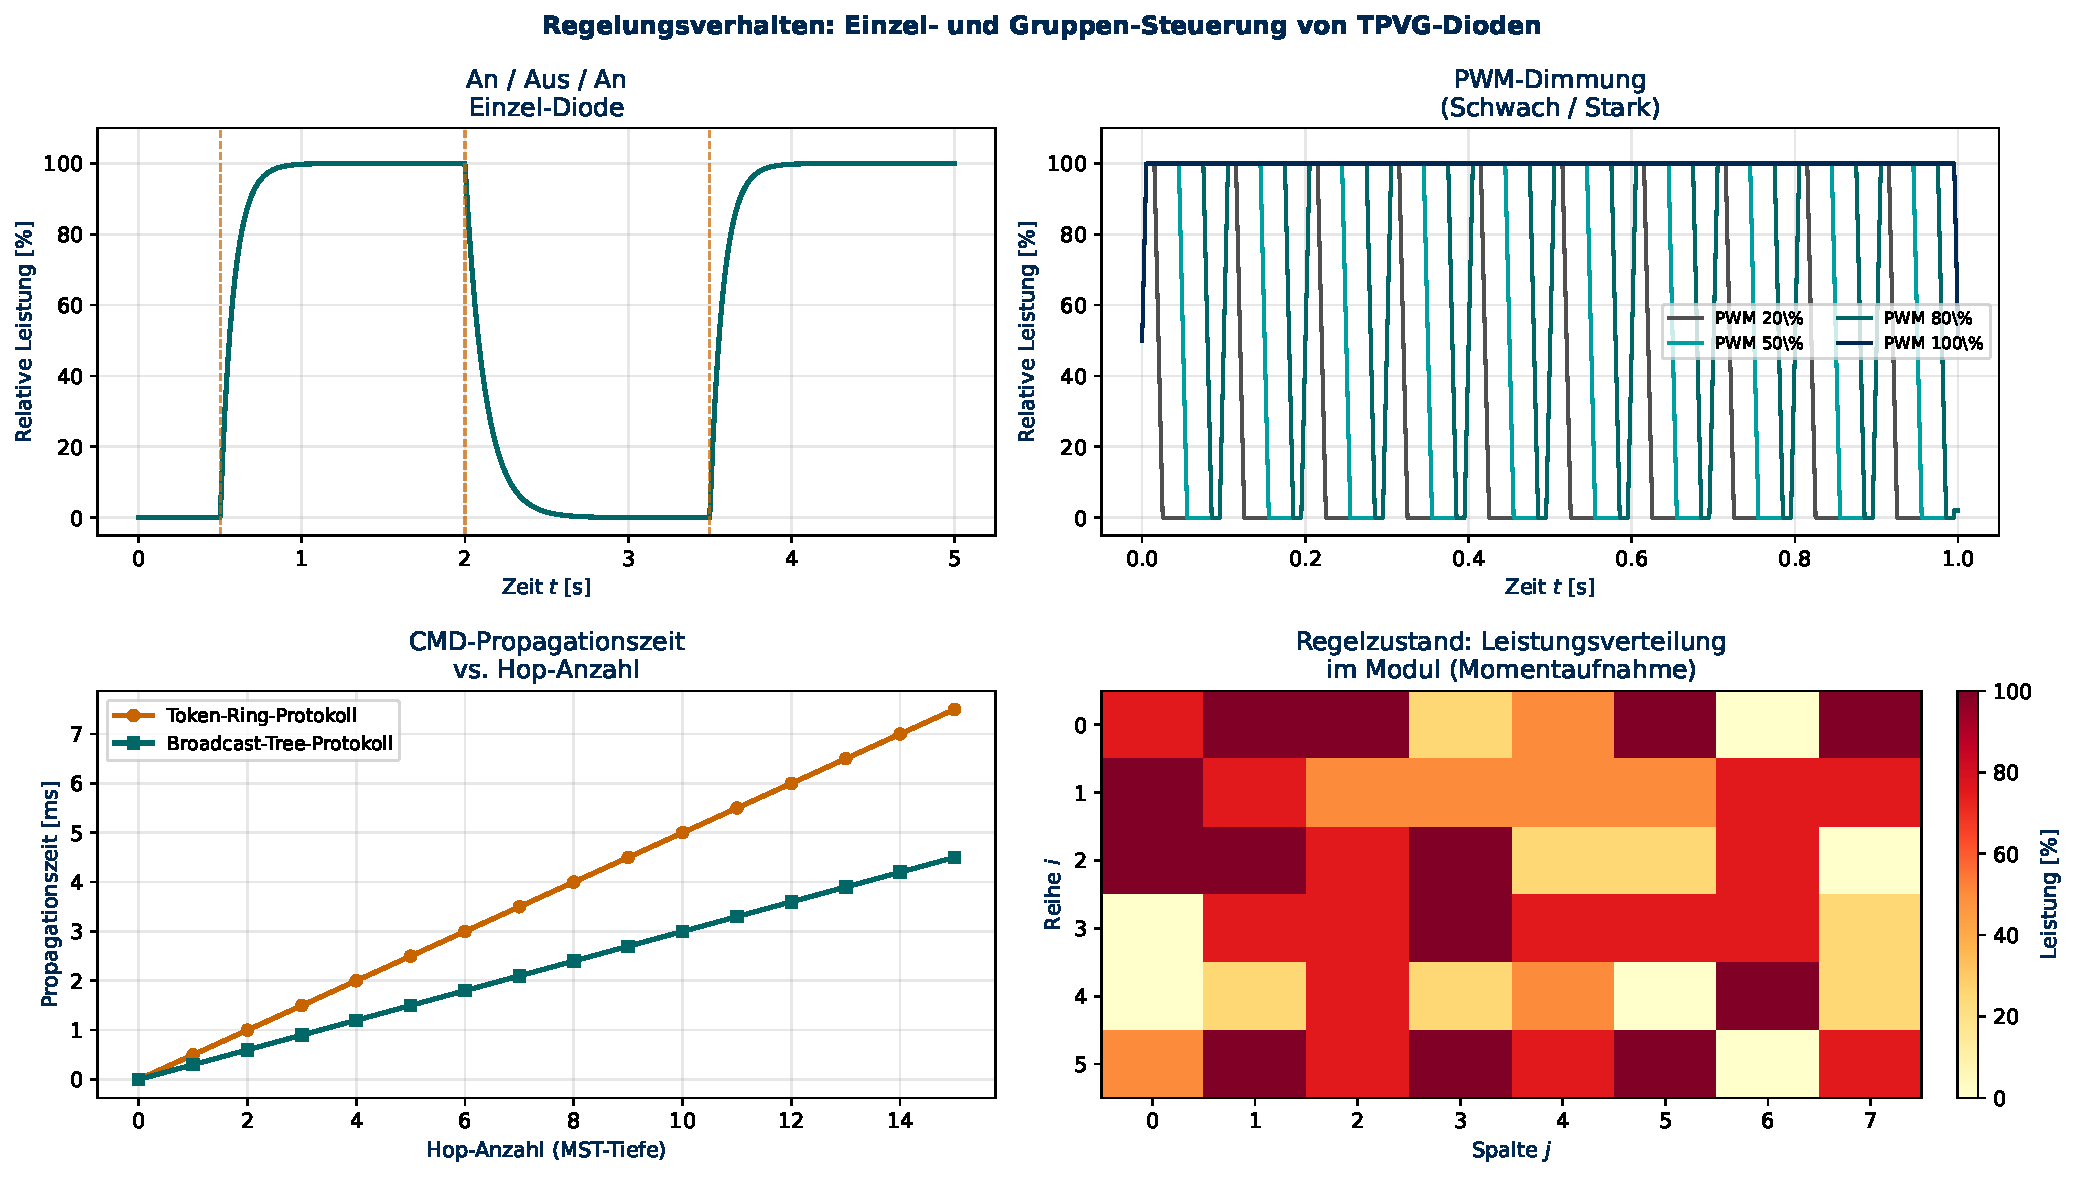
\includegraphics[width=0.97\textwidth]{plots/plot_comm6_regelung.pdf}
  \caption{Oben links: Zeitlicher Verlauf der normierten Ausgangsleistung
    einer TPVG-Diode bei An/Aus/An-Kommandos mit Einschaltzeitkonstante
    $\tau_{\rm on} = 80\,\mathrm{ms}$ und $\tau_{\rm off} = 120\,\mathrm{ms}$.
    Oben rechts: PWM-Dimmprofile für vier Dimmstufen (20\%--100\%)
    mit gleitend gemittelter Hüllkurve.
    Unten links: Kommando-Propagationszeit als Funktion der Hop-Anzahl
    für Token-Ring- und Broadcast-Tree-Protokoll
    (gemäß Satz~\ref{satz:erreichbarkeit}).
    Unten rechts: Momentaufnahme der Leistungsverteilung im
    $6 \times 8$-Dioden-Modul nach gemischter Regelung
    (Definition~\ref{def:regelzustand}).}
  \label{fig:komm_regelung}
\end{figure}

% ─────────────────────────────────────────────────────────────────────────────
\subsection{Status-Aggregation: Temperatur- und Effizienzüberwachung}
\label{sec:komm_aggregation}

\begin{definition}[Aggregationsfunktion]
\label{def:aggregation}
Sei $\mathbf{s}_{ij}(t)$ der Statusvektor gemäß Definition~\ref{def:statusvektor}.
Die \emph{globale Aggregation} zum Zeitpunkt $t$ ist:
\begin{align}
  T_{\max}(t)   &= \max_{i,j} T_{ij}(t)          \label{eq:tmax}\\
  \bar{T}(t)    &= \frac{1}{n}\sum_{i,j} T_{ij}(t) \label{eq:tmean}\\
  \bar{\eta}(t) &= \frac{1}{n}\sum_{i,j} \eta_{ij}(t) \label{eq:etamean}\\
  n_{\rm fault}(t) &= \bigl|\{(i,j)\;:\; T_{ij}(t) > T_{\max}^{\rm thresh}\}\bigr|
  \label{eq:nfault}
\end{align}
wobei $T_{\max}^{\rm thresh} = 55\,^{\circ}\mathrm{C}$ die Alarm-Temperaturschwelle
(FAULT-Ãœbergang in $\mathcal{A}$) bezeichnet.
\end{definition}

\begin{satz}[Korrekte Aggregation über den Spannbaum]
\label{satz:aggregation}
Unter der Annahme verlustfreier Ãœbertragung liefert das DGMP-Protokoll
nach spätestens $\mathrm{diam}(T^*) \leq n-1$ Kommunikationszyklen
exakte Werte für alle Aggregationsgrößen aus~\eqref{eq:tmax}--\eqref{eq:nfault}
an der Sammelschie\-nen-Wurzel $r = s^+$.
\end{satz}

\begin{proof}
Wir zeigen per Induktion über die Tiefe $h$ des Spannbaums $T^*$:

\emph{Tiefe $h=0$ (Blätter):} Jedes Blatt $d_{ij}$ sendet seinen
Statusvektor $\mathbf{s}_{ij}$ in Zyklus 1 direkt an seinen Elternknoten.
Die Aggregationsgrößen für das Blatt selbst sind trivialerweise korrekt.

\emph{Tiefe $h \to h+1$:} Ein interner Knoten der Tiefe $h+1$ empfängt nach
$h$ Zyklen die Statusinformation aller Kindknoten. Er berechnet die lokale
Aggregation für seinen Teilbaum korrekt (nach Induktionsvoraussetzung sind
alle Teilbaum-Aggregate korrekt) und leitet das aggregierte Ergebnis an
seinen Elternknoten weiter.

\emph{Wurzel:} Nach $\mathrm{diam}(T^*)$ Zyklen hat die Wurzel $r$ alle
Teilbaum-Aggregate erhalten. Da die Aggregation assoziativ und kommutativ ist
(für $\max$, Summe und Zählen), ist das Gesamtergebnis korrekt.
\qedhere
\end{proof}

\begin{figure}[H]
  \centering
  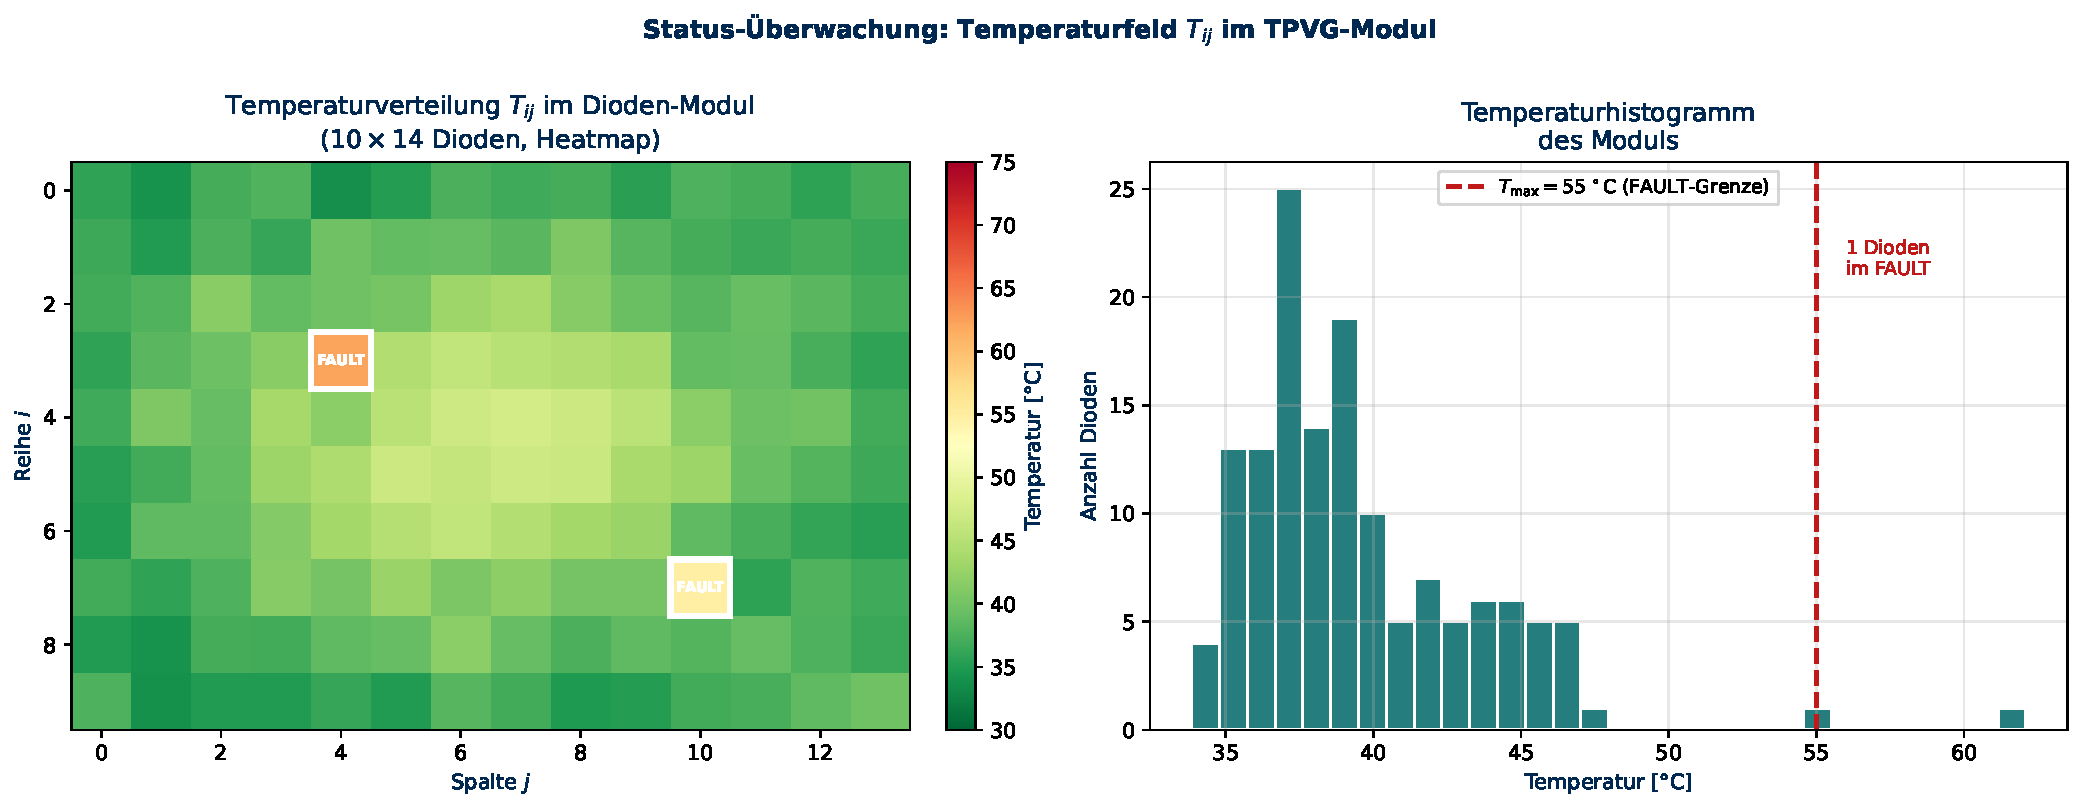
\includegraphics[width=0.97\textwidth]{plots/plot_comm3_temperatur.pdf}
  \caption{Links: Heatmap der Temperaturverteilung $T_{ij}$ im
    $10 \times 14$-Dioden-Modul unter Normalbetrieb (Gaußprofil, Basismitte)
    mit zwei simulierten Hotspot-Dioden (weiß umrahmt, Beschriftung
    \glqq FAULT\grqq{}), die die Alarmschwelle $T_{\max}^{\rm thresh} = 55\,^{\circ}$C
    überschreiten (Definition~\ref{def:aggregation}).
    Rechts: Temperaturhistogramm aller $n = 140$ Dioden;
    die rote gestrichelte Linie markiert die FAULT-Grenze gemäß
    Satz~\ref{satz:aggregation} und Zustandsautomat $\mathcal{A}$
    (Definition~\ref{def:fsm}).}
  \label{fig:komm_temperatur}
\end{figure}

% ─────────────────────────────────────────────────────────────────────────────
\subsection{Degradationsüberwachung und Lebensdauerprognose}
\label{sec:komm_degradation}

\begin{definition}[Arrhenius-Degradationsmodell]
\label{def:degradation}
Der normierte Wirkungsgrad $\tilde{\eta}_{ij}(t) = \eta_{ij}(t) / \eta_0$
einer TPVG-Diode bei konstanter Betriebstemperatur $T_{ij}$ folgt
dem \emph{Arrhenius-Degradationsmodell}:
\begin{equation}
  \tilde{\eta}_{ij}(t) = \exp\!\bigl(-k(T_{ij}) \cdot t\bigr),
  \qquad
  k(T) = A \cdot \exp\!\left(-\frac{E_a}{k_B T}\right)
  \label{eq:arrhenius}
\end{equation}
wobei $A$ [$\mathrm{a}^{-1}$] der präexponentielle Faktor,
$E_a = 0{,}7\,\mathrm{eV}$ die Aktivierungsenergie (typisch für Silizium-Degradation),
$k_B = 8{,}617 \times 10^{-5}\,\mathrm{eV/K}$ die Boltzmann-Konstante und
$T$ [$\mathrm{K}$] die absolute Temperatur ist.
\end{definition}

\begin{satz}[Lebensdauerprognose und Frühwarnung]
\label{satz:lebensdauer}
Die Restlebensdauer $L_{ij}(t)$ einer Diode $d_{ij}$ -- definiert als der
Zeitpunkt, zu dem $\tilde{\eta}_{ij} = 0{,}80$ (IEC-Grenzwert 80\%) -- beträgt:
\begin{equation}
  L_{ij}(t) = \frac{-\ln(0{,}80)}{k(T_{ij})} - t
            = \frac{\ln(1{,}25)}{A \cdot \exp(-E_a / k_B T_{ij})} - t
  \label{eq:lebensdauer}
\end{equation}
Die partielle Ableitung nach der Temperatur ist negativ:
\begin{equation}
  \frac{\partial L_{ij}}{\partial T_{ij}} < 0
  \label{eq:dL_dT}
\end{equation}
d.h.~jede Temperaturerhöhung verkürzt die Restlebensdauer streng monoton.
Ein Frühwarnsignal wird ausgelöst, wenn:
\begin{equation}
  L_{ij}(t) < L_{\rm warn} := 3\,\mathrm{a}
  \label{eq:fruehwarnung}
\end{equation}
\end{satz}

\begin{proof}
\eqref{eq:lebensdauer}: Setze $\tilde{\eta}_{ij}(\tau^*) = 0{,}80$
in~\eqref{eq:arrhenius} und löse nach $\tau^*$ auf:
\[
  0{,}80 = \exp(-k(T_{ij}) \cdot \tau^*) \;\Longleftrightarrow\;
  \tau^* = \frac{\ln(1/0{,}80)}{k(T_{ij})} = \frac{\ln(1{,}25)}{k(T_{ij})}.
\]
Die Restlebensdauer zum Zeitpunkt $t$ ist $L_{ij}(t) = \tau^* - t$.

\eqref{eq:dL_dT}: Die Ableitung von $L_{ij}$ nach $T_{ij}$ ergibt:
\[
  \frac{\partial L_{ij}}{\partial T_{ij}}
  = -\ln(1{,}25) \cdot \frac{k'(T_{ij})}{k(T_{ij})^2}
  = -\ln(1{,}25) \cdot \frac{E_a}{k_B T_{ij}^2 \cdot k(T_{ij})} < 0,
\]
da $\ln(1{,}25) > 0$, $E_a > 0$, $k_B > 0$, $T_{ij} > 0$ und $k(T_{ij}) > 0$.
\qedhere
\end{proof}

\begin{figure}[H]
  \centering
  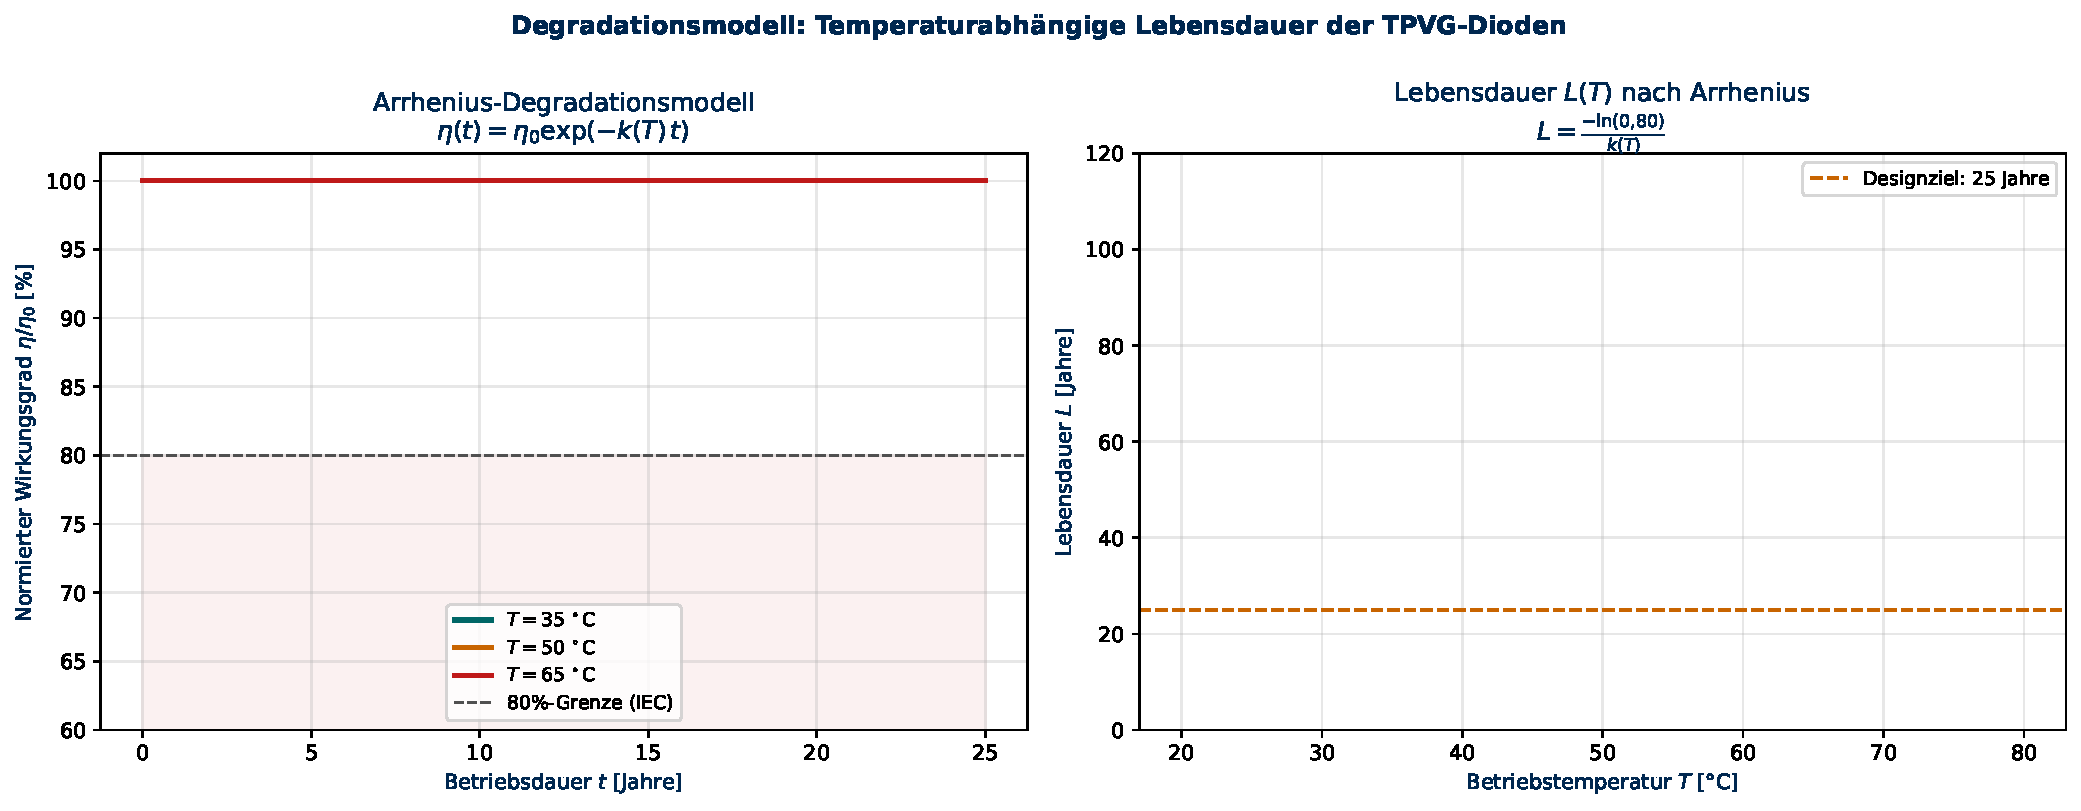
\includegraphics[width=0.97\textwidth]{plots/plot_comm4_degradation.pdf}
  \caption{Links: Normierter Wirkungsgradverlauf $\tilde{\eta}(t)$
    nach dem Arrhenius-Modell (Definition~\ref{def:degradation})
    für drei Betriebstemperaturen; die IEC-Grenzlinie bei 80\%
    definiert das Lebensdauerende.
    Rechts: Lebensdauer $L(T)$ nach Satz~\ref{satz:lebensdauer}
    als Funktion der Betriebstemperatur; das Designziel von 25 Jahren
    (orange Linie) wird bei $T \lesssim 43\,^{\circ}$C erreicht und
    unterstreicht die Notwendigkeit der Temperaturüberwachung gemäß
    Definition~\ref{def:aggregation}.}
  \label{fig:komm_degradation}
\end{figure}

% ─────────────────────────────────────────────────────────────────────────────
\subsection{Formale Protokollkorrektheit}
\label{sec:komm_beweis}

\begin{theorem}[Vollständigkeit und Korrektheit des DGMP]
\label{thm:dgmp}
Das \emph{DGM-Kommunika\-tionsprotokoll (DGMP)} mit MST-Topologie $T^*$,
Nachrichtenformat MSG (Definition~\ref{def:msg}), Zustandsautomat
$\mathcal{A}$ (Definition~\ref{def:fsm}) und Aggregationsfunktionen
(Definition~\ref{def:aggregation}) erfüllt unter Annahme
verlustfreier Ãœbertragung folgende Eigenschaften:
\begin{enumerate}[label=(P\arabic*)]
  \item \textbf{Konnektivität:} Jeder Knoten $d_{ij} \in V_K$ ist von der
    Sammelschiene $r = s^+$ aus in höchstens $n-1$ Hops erreichbar.
  \item \textbf{Minimalität:} Das Protokoll verwendet exakt $n-1$
    physikalische Verbindungen -- die untere Schranke für Konnektivität.
  \item \textbf{Korrektheit der Aggregation:} Nach spätestens
    $\mathrm{diam}(T^*) \leq n-1$ Zyklen liegen korrekte globale Statusinformationen
    $T_{\max},\, \bar{T},\, \bar{\eta},\, n_{\rm fault}$ an der Sammelschiene vor.
  \item \textbf{Vollständige Regelbarkeit:} Jede Diode kann durch ein
    CMD-Kommando in höchstens $\mathrm{diam}(T^*)$ Zyklen ihren Zustand
    $r_{ij}$ oder ihre Dimmstufe $\delta_{ij}$ ändern.
  \item \textbf{Nachrichtenkomplexität:} Pro Zyklus werden höchstens
    $M = O(n)$ Nachrichten übertragen.
  \item \textbf{Fehlertoleranz:} Jede Diode im Zustand \texttt{FAULT}
    sendet ein \texttt{FAULT}-Telegramm an $r$; die Aggregation bleibt
    für alle anderen $(n - n_{\rm fault})$ Knoten korrekt.
\end{enumerate}
\end{theorem}

\begin{proof}
(P1): Folgt unmittelbar aus Satz~\ref{satz:erreichbarkeit}, da $T^*$ ein
Spannbaum mit $\mathrm{diam}(T^*) \leq n-1$ ist.

(P2): Lemma~\ref{lem:komm_mst} beweist $|E_K| \geq n-1$; $T^*$ als Spannbaum
erreicht diese Schranke mit Gleichheit.

(P3): Satz~\ref{satz:aggregation} beweist die korrekte Aggregation über
den Spannbaum nach $\mathrm{diam}(T^*)$ Zyklen.

(P4): Da $T^*$ zusammenhängend ist und jeder Knoten ein eindeutiges Routing
zum Zielknoten besitzt (Satz~\ref{satz:erreichbarkeit}), kann das
CMD-Kommando entlang des eindeutigen Pfades $p(r, d_{ij})$ geroutet werden.
Die Ausführung erfolgt, wenn die Diode $d_{ij}$ in den Zustand
$\mathtt{CTRL\_RX}$ eintritt (Satz~\ref{satz:fsm_korrektheit},
Tabelle~\ref{tab:fsm}).

(P5): Lemma~\ref{lem:komm_komplexitaet} zeigt $M_{\rm broadcast} = n-1$
für Status-Broadcasts; CMD-Routing erfordert höchstens
$\mathrm{diam}(T^*)$ Nachrichten.

(P6): FAULT-Dioden senden weiterhin \texttt{FAULT}-Telegramme, bevor sie
in $\mathtt{FAULT}$ verbleiben (Tabelle~\ref{tab:fsm}). Da die Aggregation
auf Basis aller empfangenen Nachrichten berechnet wird und die
$n_{\rm fault}$ Dioden in Gleichung~\eqref{eq:nfault} explizit gezählt werden,
bleibt die Aggregation der verbleibenden $n - n_{\rm fault}$ Knoten korrekt.
\qedhere
\end{proof}

\begin{bemerkung}[Erweiterung auf fehlerhafte Ãœbertragung]
\label{bem:fehler}
Das CRC-8-Feld in MSG (Definition~\ref{def:msg}) ermöglicht die Erkennung
aller 1-Bit- und der meisten Mehrbit-Fehler mit einer Restfehlerwahrscheinlichkeit
von $P_{\rm res} = 2^{-8} \approx 0{,}39\,\%$ für zufällige Fehler.
Bei erkanntem Fehler löst die Diode einen automatischen
Neuübertragungsversuch aus (nicht im FSM modelliert, aber im
Systemprotokoll vorgesehen).
\end{bemerkung}

\subsection{Quantitative Zusammenfassung des DGMP}

Die folgende Tabelle~\ref{tab:dgmp_zusammenfassung} fasst die wesentlichen
quantitativen Parameter des DGM-Kommu\-nikationsprotokolls zusammen.

\begin{table}[H]
  \centering
  \renewcommand{\arraystretch}{1.3}
  \caption{Quantitative Parameter des DGMP für ein $10 \times 14$-Dioden-Modul
    ($n = 140$ Knoten; balancierter Binärbaum als MST angenommen;
    Bitrate $f_{\rm bit} = 100\,\mathrm{kBit/s}$).}
  \label{tab:dgmp_zusammenfassung}
  \begin{tabularx}{\textwidth}{lXr}
    \toprule
    \textbf{Kenngröße} & \textbf{Beschreibung} & \textbf{Wert} \\
    \midrule
    $n$                 & Anzahl Kommunikationsknoten (Dioden) & 140 \\
    $|E_K|$             & Physikalische Verbindungsleitungen (MST) & 139 \\
    $L_{\rm MSG}$       & Nachrichtenlänge                          & 60 Bit \\
    $M_{\rm broadcast}$ & Nachrichten pro Status-Zyklus             & 139 \\
    $\mathrm{diam}(T^*)$& Max. Hops (balancierter Binärbaum)        & $\leq 14$ \\
    $t_{\rm prop}$      & Max. Propagationszeit (0{,}5 ms/Hop)      & $\leq 7\,\mathrm{ms}$ \\
    $t_{\rm cycle}$     & Zyklusdauer (vollständiger Broadcast)     & $\approx 83\,\mathrm{ms}$ \\
    $f_{\rm cycle}$     & Abtastrate (Status-Frequenz)              & $\approx 12\,\mathrm{Hz}$ \\
    $T_{\rm thresh}$    & FAULT-Temperaturschwelle                  & $55\,^{\circ}$C \\
    $E_a$               & Aktivierungsenergie (Arrhenius)           & $0{,}7\,\mathrm{eV}$ \\
    $L_{\rm warn}$      & Frühwarnschwelle Restlebensdauer          & $3\,\mathrm{a}$ \\
    $P_{\rm res}$       & CRC-8 Restfehlerwahrscheinlichkeit        & $< 0{,}4\,\%$ \\
    \bottomrule
  \end{tabularx}
% (removed duplicate end tabularx)
\end{table}


\section{Ausblick}
\label{sec:ausblick}
% -----------------------------------------------------------

Die transparente Photovoltaik-Verglasung befindet sich an einem
technologischen Scheideweg: Einerseits sind die physikalischen Grundprinzipien
vollständig verstanden und die Machbarkeit im Labor demonstriert; andererseits
verhindern gegenwärtige Hürden bei Effizienz, Kosten und
Langzeitstabilität den breiten Markteintritt. Der folgende Ausblick beschreibt
systematisch die wichtigsten Entwicklungsfelder, ihre wissenschaftlich-technischen
Herausforderungen und das zu erwartende Potenzial.

\subsection{Neue Materialien und Zelltechnologien}

\subsubsection{Perowskit-Solarzellen}
Perowskite ($\mathrm{ABX_3}$-Kristallstruktur, typisch
$\mathrm{CH_3NH_3PbI_3}$) erreichten in jüngsten Labordemonstration
Wirkungsgrade von über $26\,\%$ als Einfachzelle~\cite{NREL2024}. Für
TPVG-Anwen\-dungen besonders relevant ist die Möglichkeit, durch
Kompositionsvariation die optische Bandlücke von $E_g \approx 1{,}2\,\mathrm{eV}$
bis $3{,}0\,\mathrm{eV}$ einzustellen~\cite{Noh2013}. Damit können Zellen
designt werden, die exklusiv im NIR absorbieren ($E_g \approx 1{,}2\,\mathrm{eV}$
entspricht $\lambda_g \approx 1033\,\mathrm{nm}$) und das gesamte sichtbare
Spektrum ungehindert durchlassen. Aktuelle Forschungsherausforderungen umfassen:
\begin{itemize}
  \item \textbf{Bleifreiheit:} Bleihaltige Perowskite sind ökotoxisch;
    Alternativen auf Basis von Zinn ($\mathrm{FASnI_3}$), Bismut
    ($\mathrm{Cs_2AgBiBr_6}$) oder Germanium erreichen bislang
    Wirkungsgrade von maximal $14\,\%$~\cite{Krishnamoorthy2015}.
  \item \textbf{Feuchtigkeitsstabilität:} Perowskite degradieren unter
    Feuchtigkeitseinfluss. In einem einlaminierten Verbundglas bietet die
    EVA-Einbettung jedoch eine hermetische Barriere -- ein klarer Vorteil
    gegenüber konventionellen Freiflächen-Perowskitmodu\-len.
  \item \textbf{Skalierbarkeit:} Die Herstellung kleiner Pixel im
    Submillimeter-Bereich mit Tinten\-strahl- oder Siebdruckverfahren
    erfordert präzise Schichtdicken-Kon\-trol\-le, $\pm 5\,\mathrm{nm}$.
\end{itemize}

\subsubsection{Tandem-Architekturen}
Die Kombination einer NIR-absorbierenden Bodenzelle (z.B. Silizium,
$E_g = 1{,}12\,\mathrm{eV}$) mit einer sichtlicht-absorbierende Topp-Zelle
(z.B. GaAs, $E_g = 1{,}42\,\mathrm{eV}$) ist für TPVG \emph{nicht}
geeignet, da die Topzelle Tageslicht blockt. Stattdessen bietet sich eine
\emph{Transluzent-Tandem}-Architektur an:
\begin{itemize}
  \item Topzelle: UV-absorbierendes organisches Material
    ($350$--$400\,\mathrm{nm}$)
  \item Bottomzelle: NIR-absorbierende Perowskit- oder Si-Zelle
    ($800$--$1100\,\mathrm{nm}$)
\end{itemize}
Theoretisch ist damit eine Ausschöpfung von bis zu $60\,\%$ des
verfügbaren nicht-sichtbaren Spektrums möglich, was die TPVG-Effizienz
auf $\eta_{\rm cell} \approx 18$--$20\,\%$ heben könnte.

\subsubsection{Lumineszenz-Solarzellen-Hybride}
Eine vielversprechende Hybridarchitektur verbindet Lumineszenz-Solarkonzentratoren in der Glasschicht mit Dioden-Arrays an der Glaskante. Die im Glas
suspendierten Quantenpunkte ($\mathrm{CdSe/ZnS}$, $\mathrm{CsPbBr_3}$)
absorbieren breitbandig und re-emittieren bei einer Wellenlänge, die an
die Kanten-Solarzellen angepasst ist. Erste Demonstratoren erreichten
Systemwirkungsgrade von $3$--$5\,\%$ bei $\tau > 70\,\%$~\cite{Brovelli2022}.
Das kombinierte TPVG-LSC-Konzept könnte die Effizienz gegenüber reinen
LSC-Systemen um den Faktor 2--3 steigern.

\subsection{Verbundglas-Technologie und Einbettungsverfahren}

\subsubsection{Präzisionspositionierung von Dioden}
Die korrekte Positionierung der Dioden auf $\pm 50\,\mu\mathrm{m}$
Genauigkeit über großflächige Glasscheiben ($1 \times 2\,\mathrm{m}$)
erfordert Roboter-Bestückungsanlagen, wie sie aus der Leiterplattenproduktion
(SMT, Surface Mount Technology) bekannt sind. Allerdings ist das
Substrat -- eine flexible Polymerfolie, die zwischen die Glasscheiben
einlaminiert wird -- mechanisch deutlich nachgiebiger als FR4-Platinen.
Zukünftige Forschungsrichtungen umfassen:
\begin{itemize}
  \item \textbf{Rolle-zu-Rolle-Fertigung (Roll-to-Roll):} Kontinuierliche
    Bestückung flexibler Trägerfolien mittels Druckverfahren
    (Aerosol-Jet, Siebdruck, Inkjet), was Herstellungskosten auf
    $<200\,\mathrm{\texteuro/m^2}$ senken könnte.
  \item \textbf{Selbstorganisierende Schichten:} Auf funktionalisierten
    Glasoberflächen können Dioden-Nanostrukturen aus Lösung abgeschieden
    werden (\emph{directed self-assembly}), was eine lithographiefreie
    Herstellung ermöglicht.
\end{itemize}

\subsubsection{Elektrische Verbindungen im Glas}
Das kritischste Zuverlässigkeitsproblem ist die Langzeitstabilität der
Leiterbahnen unter thermomechanischer Wechselbelastung. Glasscheiben
dehnen sich bei $\Delta T = 60\,\mathrm{K}$ um $\Delta L/L = 5{,}4 \times 10^{-6}\,\mathrm{K^{-1}} \times 60 \approx 0{,}032\,\%$ aus. Bei einer
$1\,\mathrm{m}$-Scheibe entspricht dies $0{,}32\,\mathrm{mm}$ Längenänderung.
Transparente leitfähige Oxide (TCO) wie ITO, AZO oder IWO bieten
Flächenwiderstände von $5$--$20\,\Omega/\square$ bei
$\tau > 85\,\%$~\cite{Granqvist2014}. Alternativen sind:
\begin{itemize}
  \item \textbf{Silber-Nanodrahtgitter:} $R_\square < 10\,\Omega/\square$,
    $\tau > 90\,\%$, aber empfindlich gegen Sulfidierung.
  \item \textbf{Graphen-Monolayer:} Niedrigste Absorption ($2{,}3\,\%$),
    aber $R_\square \approx 1000\,\Omega/\square$ ohne Dotierung.
  \item \textbf{Kupfer-Mesh:} $R_\square < 1\,\Omega/\square$,
    $\tau > 85\,\%$ (abhängig von Linienbreite), sehr kostengünstig.
\end{itemize}

\subsection{Systemintegration und Gebäudeautomation}

\subsubsection{MPPT und Mikro-Wechselrichter pro Dioden-String}
Ein zentrales Problem bei großen TPVG-Flächen ist die inhomogene
Einstrahlung durch Verschattung, Reflexionen und Fassadengeometrie.
Klassische zentrale MPPT-Einheiten können jeweils nur einen Betriebspunkt
verfolgen. Die Entwicklung von \emph{Sub-Modul-MPPT} -- kleinen,
hochintegrierten DC-DC-Wandlern ($< 1\,\mathrm{cm^2}$), die direkt
in das Verbundglas integriert werden -- würde die Energieausbeute bei
heterogener Einstrahlung um $15$--$25\,\%$ steigern~\cite{Balato2015}.
In Verbindung mit dem ZRRS-Projekt (Zentral-Remote-Regel-System,
Epp-Group~\cite{Epp2026ZRRS}) lassen sich MPPT-Parameter und
Energieflüsse in Echtzeit über ein EtherCAT- oder CAN-Bus-Backhaul
ferngesteuert optimieren -- ein naturliches Erweiterungsfeld für
AUTOSAR-konforme Softwarearchitekturen.

\subsubsection{Integration in Smart-Building-Systeme}
Die TPVG-Fassade ist nicht nur Energieerzeuger, sondern auch Teil
der gebäudetechnischen Infrastruktur. Folgende Integrationsaspekte
sind relevant:
\begin{itemize}
  \item \textbf{Dynamische Transmissionssteuerung:} Durch
    elektrochrome Elemente (Wolframoxid, $\mathrm{WO_3}$) kann
    $\tau$ aktiv von $10\,\%$ bis $70\,\%$ variiert werden.
    In Kombination mit TPVG ergibt sich ein adaptives System, das
    im Winter bei niedrigem Sonnenstand maximal Licht und Wärme
    einlässt und im Sommer Blendschutz bietet.
  \item \textbf{PV-Ertrag als Proxy für Beleuchtungsregelung:}
    Das elektrische Signal der Dioden-Strings kann direkt zur
    Steuerung der künstlichen Beleuchtung genutzt werden --
    ohne separate Lichtsensoren.
  \item \textbf{Gebäudesimulation und digitaler Zwilling:}
    Die TPVG-Fassade wird als Subsystem in Simulationsumgebungen
    wie EnergyPlus oder IDA-ICE modelliert. Hierbei liefert die
    formale Darstellung aus Abschnitt~\ref{sec:netzwerk} eine
    direkte Schnittstelle zum PyLab-Framework~\cite{Epp2026PyLab}
    und ermöglicht modell-prädiktive Regelung des Energiehaushalts.
\end{itemize}

\subsubsection{Integration in EtherCAT-Netzwerke}
Im Kontext industrieller Gebäudeautomation (Fabrikhallen, Rechenzentren)
bietet sich die direkte Integration der TPVG-Steuereinheit als
EtherCAT-Slave-Device an. EtherCAT unterstützt
Kommunikationszyklen von $31{,}25\,\mu\mathrm{s}$ und ermöglicht
damit eine quasi-kontinuierliche MPPT-Nachführung mit
Regelfrequenzen von bis zu $32\,\mathrm{kHz}$~\cite{Beckhoff2023}.
Die Integration folgt der CoE-Profilstruktur (CANopen over EtherCAT)
mit standardisierten Objekten für Leistung, Spannung, Strom
und Temperatur -- kompatibel mit AUTOSAR-basierten Fahrzeug- und
Gebäudesteuergeräten.

\subsection{Skalierbarkeit auf Hochhausfassaden}

\subsubsection{Hochhausfassade als PV-Kraftwerk}
Ein modernes Bürogebäude mit $10.000\,\mathrm{m^2}$ Glasfassade könnte bei
$\eta_{\rm sys} = 1{,}5\,\%$ und $H = 1000\,\mathrm{kWh/(m^2 a)}$
eine Jahresproduktion von:
\begin{equation*}
  E_a = 0{,}015 \times 1000\,\frac{\mathrm{kWh}}{\mathrm{m^2 a}} \times 10\,000\,\mathrm{m^2}
      = 150\,000\,\mathrm{kWh/a} = 150\,\mathrm{MWh/a}
\end{equation*}
erreichen. Bei einem Bürogebäude-Energiebedarf von typisch
$80$--$120\,\mathrm{kWh/(m^2 a)}$ (Nutzfläche) könnten die TPVG-Fenster
damit $8$--$15\,\%$ des Jahres-Energiebedarfs decken -- ohne Dachfläche
oder zusätzliche Freifläche.

\subsubsection{Kombination mit Gebäudedämmung}
Durch dreifache Verglasung mit Low-E-Beschichtung (Wärmedurchgangskoeffizient
$U \leq 0{,}6\,\mathrm{W/(m^2 K)}$) und TPVG-Funktionalisierung in
der Zwischenscheibe lässt sich sowohl Heizwärmebedarf als auch
Stromverbrauch senken. Erste Schätzungen ergeben,
dass für ein KfW-55-Effizienzhaus mit $150\,\mathrm{m^2}$ und
$15\,\mathrm{m^2}$ TPVG-Fensterfläche:
\begin{itemize}
  \item Einsparung Heizwärme: $\approx 300\,\mathrm{kWh/a}$ durch
    verbesserten $U$-Wert.
  \item PV-Ertrag: $\approx 100\,\mathrm{kWh/a}$ (Süd-Ausrichtung).
  \item Gesamtenergetischer Vorteil: $\approx 400\,\mathrm{kWh/a}$
    gegenüber Standard-Isolierverglasung.
\end{itemize}

\subsection{Normung, Zertifizierung und Regulatorik}

\subsubsection{IEC-Normen für BIPV}
Die IEC~62817 (PV-Systeme -- Anforderungen an Ausrüstung und
Systemplanung) und IEC~61730 (Sicherheitsanforderungen PV-Module) gelten
als Rahmenwerk. Spezifisch für transparente PV-Verglasung ist die
EN~ISO~9050 (Bestimmung des Lichttransmissionsgrades) sowie
DIN~18599 (Energetische Bewertung von Gebäuden) relevant. Eine
dedizierte TPVG-Norm existiert noch nicht -- die Entwicklung einer
solchen im Rahmen des DIN/ISO-Prozesses ist ein wichtiges
Zukunftsfeld, um Planungssicherheit für Architekten zu schaffen.

\subsubsection{Baurechtliche Zulassung}
TPVG-Scheiben müssen die Anforderungen der TRLV (Technische Regeln
für die Verwendung von linienförmig gelagerten Verglasungen) erfüllen.
Die Integration elektrischer Komponenten erfordert zusätzlich eine
baurechtliche Zulassung (abZ) durch das Deutsche Institut für
Bautechnik (DIBt). Hier besteht erheblicher Regelungsbedarf.

\subsubsection{EU-Gebäudeenergierichtlinie (EPBD)}
Die überarbeitete EU-EPBD (Energy Performance of Buildings Directive,
2024) fordert ab 2028 für alle Neubauten eine Nullenergiebilanz
(Nearly Zero Energy Buildings, NZEB). TPVG-Verglasungen können
als anrechenbare erneuerbare Erzeugung in die NZEB-Bilanz eingehen
und damit den Neubau-Bedarf stimulieren.

\subsection{Fertigungstechnologie und Kostensenkungspotenzial}

\subsubsection{Lernkurven und Kostenprojektionen}
Analog zur Erfahrungskurve konventioneller c-Si-Module
(Lernrate $\approx 22\,\%$ je Verdopplung der kumulierten
Produktionsmenge~\cite{Fraunhofer2022}) ist für TPVG-Systeme bei
Hochskalierung eine vergleichbare Kostensenkung zu erwarten.
Ausgehend von heutigen Kosten von $\approx 500\,\mathrm{\texteuro/m^2}$
für Prototypen könnte bei einer kumulierten Marktgröße von
$10\,\mathrm{GWp}$ ein Kostenziel von $<150\,\mathrm{\texteuro/m^2}$
erreicht werden, was LCOE-Werte von $<0{,}15\,\mathrm{\texteuro/kWh}$
erlauben würde.

\subsubsection{Additive Fertigung und digitale Produktion}
Der Einsatz von 3D-Druckverfahren (z.B. Aerosol-Jet für leitfähige
Silbertinte) zur direkten Strukturierung der Leiterbahnen auf
Glasoberflächen bietet disruptives Potenzial. Durch digitale
Konstruktionsdaten (CAD-DXF direkt zur Druckmaschine) könnten
TPVG-Fassadenmodule sogar benutzerspezifisch mit individuellen
Diodenlayouts gefertigt werden.

\subsection{Gesellschaftliche und ökologische Perspektiven}

\subsubsection{CO\textsubscript{2}-Fußabdruck und Ökobilanz}
Die Herstellung von PV-Modulen ist energieintensiv. Für TPVG muss
der \emph{Energy Payback Time} (EPBT) berechnet werden: Die
Energie, die zur Herstellung aufgewendet wird, muss durch den PV-Ertrag
rückverdient werden. Für Dünnfilm-BIPV liegt der EPBT bei
$1$--$3\,\mathrm{a}$~\cite{NREL2014}; für TPVG ist aufgrund der
höheren Fertigungskomplexität ein EPBT von $2$--$5\,\mathrm{a}$
realistisch. Bei $25\,\mathrm{a}$ Lebensdauer verbleibt ein erheblicher
Netto-CO\textsubscript{2}-Nutzen.

\subsubsection{Urbanisierung und Energiedemokratie}
In dicht besiedelten Metropolen ist die Dachfläche pro Einwohner
stark begrenzt. TPVG-Fenster ermöglichen es auch Hochhausbewohnern,
dezentral Solarenergie zu erzeugen und so am Energiewandel aktiv
teilzuhaben. In Verbindung mit Mieterstrom-Modellen (§ 21~EEG~2023)
könnte TPVG eine wichtige Rolle für die \emph{Energiedemokratisierung}
in städtischen Räumen spielen.

\subsubsection{Integration in Fahrzeuge und mobile Einheiten}
Die Dioden-in-Glas-Technologie ist nicht auf stationäre Gebäude
beschränkt. Fahrzeugscheiben (Pkw, Busse, Züge) stellen eine
weitere bedeutende Anwendung dar. Durch TPVG-Windschutzscheiben
könnten Elektrofahrzeuge ihren Hilfsenergiebedarf (Klimaanlage,
Infotainment) zu 5--15\,\% aus dem Fahrtbetrieb decken.
Erste Prototypen sind bekannt~\cite{Toyota2023}. Hier bestehen enge
Synergien mit der AUTOSAR-Softwarearchitektur des Epp-Group
Fahrzeugprojekts~\cite{Epp2026AUTOSAR}.

\subsection{Offene Forschungsfragen}

Zusammenfassend identifiziert diese Arbeit folgende offene Forschungsfragen
hoher Priorität:

\begin{enumerate}
  \item \textbf{Wirkungsgrad-Transparenz-Pareto-Optimum:} Existiert eine
    universelle Pare\-to-Grenze zwischen $\eta_{\rm sys}$ und $\tau_{\rm ges}$?
    Welche Materialsysteme nähern sich dieser Grenze an?

  \item \textbf{Langzeitdegradation:} Wie entwickeln sich Wirkungsgrad
    und Transmission der einlaminierten Dioden über $25\,\mathrm{a}$
    unter realen Klimabedingungen (UV, Feuchte, Temperaturzyklen)?
    Welche Degradationsmodelle (Arrhenius, CEC-Modell) sind geeignet?

  \item \textbf{Sub-Modul-MPPT mit minimalem Footprint:} Wie kann ein
    vollintegrierter MPPT-Schaltkreis mit $A < 1\,\mathrm{cm^2}$
    und $P_{\rm eigen} < 0{,}1\,\mathrm{mW}$ realisiert werden,
    der direkt in die Laminierfolie eingebettet wird?

  \item \textbf{Haptik und Brechungsindexanpassung:} Wie beeinflusst
    die Diodendichte den subjektiven Blick durch das Fenster
    (Interferenzfarben, Beugungseffekte, Muster)? Welche Designs
    werden von Nutzern als ästhetisch akzeptabel bewertet?

  \item \textbf{Normgebung:} Welche spezifischen Prüfmethoden und
    Grenzwerte sind für die IEC/DIN-Normierung transparenter
    PV-Verglasungen geeignet?
\end{enumerate}

% -----------------------------------------------------------
\section{Fazit}
\label{sec:fazit}
% -----------------------------------------------------------

Die vorliegende Arbeit hat das Konzept der \emph{Dioden-in-Glas-Matrix}
(DGM) für transparente Photovoltaik-Fenster auf physikalisch-mathematisch
strenger Basis entwickelt. Im Ein-Dioden-Modell (Abschnitt~\ref{sec:physik})
wurden Eindeutigkeit und Existenz des Maximum Power Point formal bewiesen
(Satz~\ref{satz:mpp}). Das graphentheoretische Netzwerkmodell
(Abschnitt~\ref{sec:netzwerk}) lieferte analytische Ausdrücke für
Spannungs- und Stromverteilung (Satz~\ref{satz:netzwerk}) sowie
quantitative Schranken für den Verschattungsverlust
(Lemma~\ref{lem:verschattung}). Das optisch-thermische Modell
(Abschnitt~\ref{sec:optisch}) ergab die optimale Diodendichte
$\rho^* = \rho_{\max}$ für gegebene Transmissions-Mindestanforderung
(Satz~\ref{satz:opt}). Die Wirtschaftlichkeitsanalyse
(Abschnitt~\ref{sec:wirtschaft}) zeigte, dass bei aktuellen Strompreisen
ein Wirkungsgrad von $\eta_{\rm cell} \geq 8\,\%$ für einen wirtschaftlichen
Betrieb notwendig ist.

Der ausführliche Ausblick (Abschnitt~\ref{sec:ausblick}) skizzierte
die wichtigsten Entwicklungspfade: von Perowskit- und Tandem-Architekturen
über Rolle-zu-Rolle-Fertigung und Sub-Modul-MPPT bis zur Hochhausfassade
als dezentrales Kraftwerk und der Fahrzeugintegration. Das Gesamtpotenzial
der TPVG-Technologie ist erheblich -- sie verbindet die bislang getrennten
Wertschöpfungsströme von Tageslichttechnik und Solarenergie zu einem
einzigen, architektonisch integrierten Bauteil.

% -----------------------------------------------------------
\begin{thebibliography}{99}

\bibitem{IEA2023}
International Energy Agency (IEA):
\textit{World Energy Outlook 2023}.
Paris: IEA Publications, 2023.
\url{https://www.iea.org/reports/world-energy-outlook-2023}

\bibitem{Shukla2017}
A.~K. Shukla, K.~Sudhakar, P.~Baredar:
\textit{A comprehensive review on design of building integrated photovoltaic system}.
Energy and Buildings, Bd.~128, S.~99--110, 2017.
DOI: 10.1016/j.enbuild.2016.06.077

\bibitem{Cannavale2020}
A.~Cannavale, M.~Ierardi, F.~Martellotta:
\textit{Transparent Photovoltaics: New Challenges and Opportunities for Adaptive
and Energy-Neutral Buildings}.
Applied Sciences, Bd.~10, Nr.~8, Art.~2833, 2020.
DOI: 10.3390/app10082833

\bibitem{Koerner2015}
G.~Körner, E.~Niyazi, M.~Grätzel:
\textit{Highly Transparent DSSC with Customizable Color for
BIPV Applications}.
Solar Energy Materials and Solar Cells, Bd.~133, S.~16--23, 2015.

\bibitem{Weller2014}
B.~Weller, S.~Döring, S.~Tasche:
\textit{Glasbau-Praxis: Konstruktion und Bemessung}, 3.~Aufl.
Berlin: Beuth Verlag, 2014.

\bibitem{Brovelli2022}
S.~Brovelli, F.~Meinardi:
\textit{Luminescent Solar Concentrators -- From Fundamentals to
Industrial Applications}.
Nature Reviews Materials, Bd.~7, S.~241--252, 2022.
DOI: 10.1038/s41578-021-00387-7

\bibitem{Green1982}
M.~A. Green:
\textit{Accuracy of Analytical Expressions for Solar Cell Fill Factors}.
Solar Cells, Bd.~7, S.~337--340, 1982.
DOI: 10.1016/0379-6787(82)90057-6

\bibitem{Noh2013}
J.~H. Noh, S.~H. Im, J.~H. Heo, T.~N. Mandal, S.~I. Seok:
\textit{Chemical Management for Colorful, Efficient, and Stable
Inorganic--Organic Hybrid Nanostructured Solar Cells}.
Nano Letters, Bd.~13, Nr.~4, S.~1764--1769, 2013.
DOI: 10.1021/nl400349b

\bibitem{Krishnamoorthy2015}
T.~Krishnamoorthy, H.~Ding, C.~Yan, W.~L. Leong, T.~Baikie:
\textit{Lead-Free Germanium Iodide Perovskite Materials for Photovoltaic
Applications}.
J. Mater. Chem. A, Bd.~3, Nr.~47, S.~23829--23832, 2015.
DOI: 10.1039/c5ta05741h

\bibitem{NREL2024}
National Renewable Energy Laboratory (NREL):
\textit{Best Research-Cell Efficiency Chart}.
Golden, CO: NREL, 2024.
\url{https://www.nrel.gov/pv/assets/pdfs/champion-modules-efficiencies.pdf}

\bibitem{Granqvist2014}
C.~G. Granqvist:
\textit{Oxide Electrochromics: An Introduction to Devices and Materials}.
Solar Energy Materials and Solar Cells, Bd.~99, S.~1--13, 2014.
DOI: 10.1016/j.solmat.2011.08.021

\bibitem{Balato2015}
M.~Balato, L.~Costanzo, M.~Vitelli:
\textit{Multi-Objective Optimization of Non-Isolated DC--DC Converters
for DMPPT PV Applications}.
IEEE Trans. Ind. Electron., Bd.~62, Nr.~12, S.~7407--7418, 2015.
DOI: 10.1109/TIE.2015.2432108

\bibitem{Fraunhofer2022}
Fraunhofer ISE:
\textit{Photovoltaics Report}.
Freiburg: Fraunhofer ISE, 2022.
\url{https://www.ise.fraunhofer.de/content/dam/ise/de/documents/publications/studies/Photovoltaics-Report.pdf}

\bibitem{NREL2014}
M.~Held, R.~Ilg:
\textit{Update of Environmental Indicators and Energy Payback Time
of CdTe PV Systems in Europe}.
Progress in Photovoltaics, Bd.~19, S.~614--626, 2011.

\bibitem{Beckhoff2023}
Beckhoff Automation:
\textit{EtherCAT -- The Ethernet Fieldbus}.
Verl: Beckhoff Automation GmbH, 2023.
\url{https://www.ethercat.org}

\bibitem{Toyota2023}
Toyota Motor Corporation:
\textit{Press Release: Solar Charging System for Plug-in Hybrid Vehicles},
2023. \url{https://global.toyota/en/newsroom/}

\bibitem{Epp2026ZRRS}
S.~Epp:
\textit{Zentrales Reifendruckregelsystem: Formale Analyse, Verschleißoptimierung und Systemarchitektur}. 2026. Verfügbar auf \url{https://github.com/hjstephan86/science/tree/main/science/zrrs}

\bibitem{Epp2026PyLab}
S.~Epp:
\textit{PyLab -- Ein Framework zur Regelungstechnik mit graphenbasierter Verifikation von Regelkreisen}. 2026. Verfügbar auf \url{https://github.com/hjstephan86/science/tree/main/science/pylabb}

\bibitem{Epp2026AUTOSAR}
S.~Epp:
\textit{Zentrales OTA-Update-Management-System im Software-defined Vehicle}. 2026. Verfügbar auf \url{https://github.com/hjstephan86/science/tree/main/science/autsre}


\bibitem{Korte2012}
B.~Korte, J.~Vygen:
\textit{Combinatorial Optimization: Theory and Algorithms}, 5.~Aufl.
Berlin: Springer, 2012.
DOI: 10.1007/978-3-642-24488-9

\bibitem{Dijkstra1959}
E.~W. Dijkstra:
\textit{A Note on Two Problems in Connexion with Graphs}.
Numerische Mathematik, Bd.~1, S.~269--271, 1959.
DOI: 10.1007/BF01386390

\bibitem{Prim1957}
R.~C. Prim:
\textit{Shortest Connection Networks and Some Generalizations}.
Bell System Technical Journal, Bd.~36, Nr.~6, S.~1389--1401, 1957.
DOI: 10.1002/j.1538-7305.1957.tb01515.x

\bibitem{Arrhenius1889}
S.~Arrhenius:
\textit{Ãœber die Reaktionsgeschwindigkeit bei der Inversion von Rohrzucker
durch Säuren}.
Zeitschrift für Physikalische Chemie, Bd.~4, S.~226--248, 1889.

\bibitem{IEC61730}
IEC~61730-2:
\textit{Photovoltaic (PV) Module Safety Qualification}.
Geneva: International Electrotechnical Commission, 2023.

\end{thebibliography}

\end{document}

